\section{sim-zesto.cpp File Reference}
\label{sim-zesto_8cpp}\index{sim-zesto.cpp@{sim-zesto.cpp}}
{\tt \#include $<$stdio.h$>$}\par
{\tt \#include $<$stdlib.h$>$}\par
{\tt \#include $<$math.h$>$}\par
{\tt \#include $<$signal.h$>$}\par
{\tt \#include $<$unistd.h$>$}\par
{\tt \#include $<$sys/io.h$>$}\par
{\tt \#include \char`\"{}zesto-qsim.h\char`\"{}}\par
{\tt \#include \char`\"{}host.h\char`\"{}}\par
{\tt \#include \char`\"{}misc.h\char`\"{}}\par
{\tt \#include \char`\"{}machine.h\char`\"{}}\par
{\tt \#include \char`\"{}regs.h\char`\"{}}\par
{\tt \#include \char`\"{}memory.h\char`\"{}}\par
{\tt \#include \char`\"{}loader.h\char`\"{}}\par
{\tt \#include \char`\"{}syscall.h\char`\"{}}\par
{\tt \#include \char`\"{}options.h\char`\"{}}\par
{\tt \#include \char`\"{}stats.h\char`\"{}}\par
{\tt \#include \char`\"{}sim.h\char`\"{}}\par
{\tt \#include \char`\"{}thread.h\char`\"{}}\par
{\tt \#include \char`\"{}zesto-opts.h\char`\"{}}\par
{\tt \#include \char`\"{}zesto-core.h\char`\"{}}\par
{\tt \#include \char`\"{}zesto-oracle.h\char`\"{}}\par
{\tt \#include \char`\"{}zesto-fetch.h\char`\"{}}\par
{\tt \#include \char`\"{}zesto-decode.h\char`\"{}}\par
{\tt \#include \char`\"{}zesto-bpred.h\char`\"{}}\par
{\tt \#include \char`\"{}zesto-alloc.h\char`\"{}}\par
{\tt \#include \char`\"{}zesto-exec.h\char`\"{}}\par
{\tt \#include \char`\"{}zesto-commit.h\char`\"{}}\par
{\tt \#include \char`\"{}zesto-uncore.h\char`\"{}}\par
{\tt \#include \char`\"{}zesto-cache.h\char`\"{}}\par
{\tt \#include \char`\"{}machine.def\char`\"{}}\par


Include dependency graph for sim-zesto.cpp:\nopagebreak
\begin{figure}[H]
\begin{center}
\leavevmode
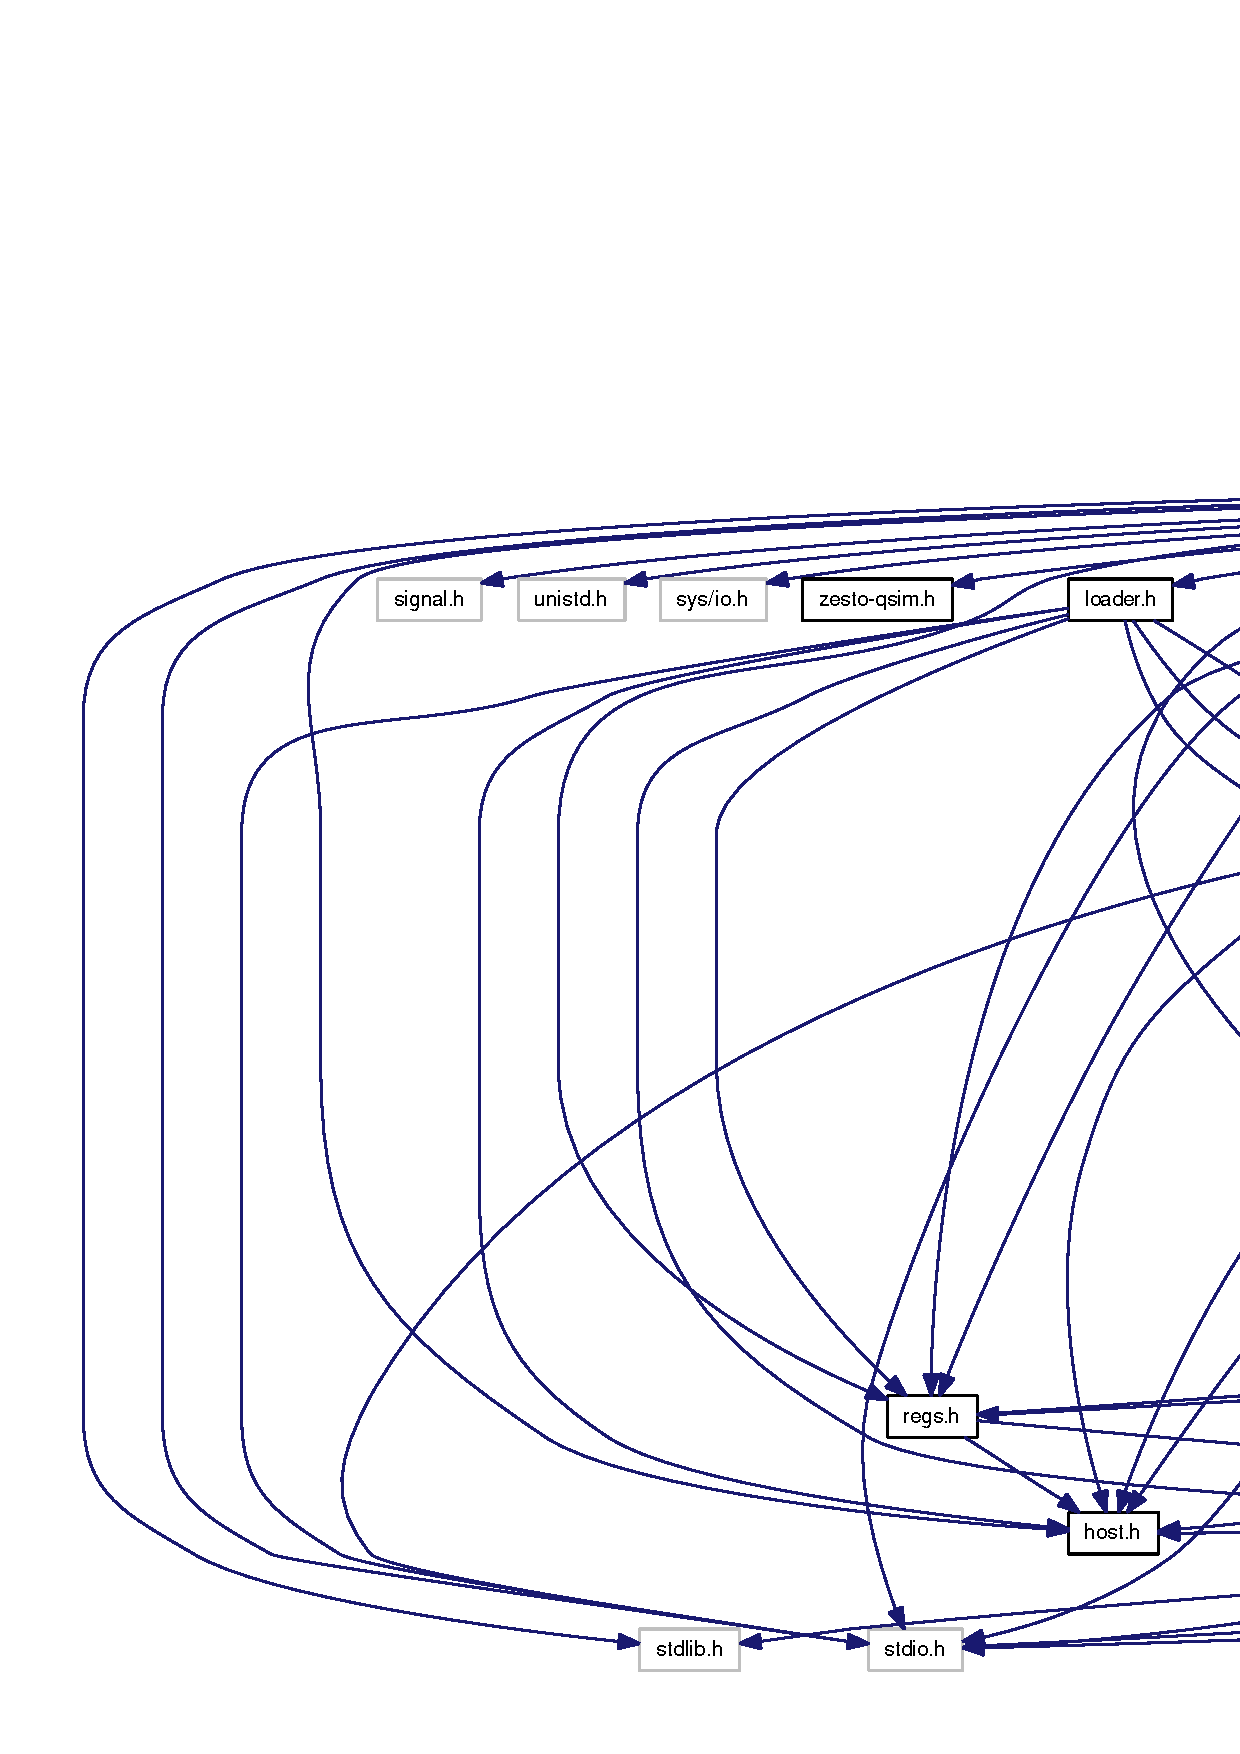
\includegraphics[width=420pt]{sim-zesto_8cpp__incl}
\end{center}
\end{figure}
\subsection*{Defines}
\begin{CompactItemize}
\item 
\#define {\bf SET\_\-NPC}(EXPR)~(thread $\rightarrow$ regs.regs\_\-NPC = (EXPR))
\item 
\#define {\bf CPC}~(thread $\rightarrow$ regs.regs\_\-PC)
\item 
\#define {\bf CPC}~(thread $\rightarrow$ regs.regs\_\-PC)
\item 
\#define {\bf NPC}~(thread $\rightarrow$ regs.regs\_\-NPC)
\item 
\#define {\bf SET\_\-NPC}(EXPR)~(thread $\rightarrow$ regs.regs\_\-NPC = (EXPR))
\item 
\#define {\bf SET\_\-NPC\_\-D}(EXPR)~SET\_\-NPC(EXPR)
\item 
\#define {\bf SET\_\-NPC\_\-V}(EXPR)~((Mop $\rightarrow$ fetch.inst.mode \& MODE\_\-OPER32) ? SET\_\-NPC((EXPR)) : SET\_\-NPC((EXPR) \& 0xffff))
\item 
\#define {\bf \_\-HI}(N)~((N) \& 0x04)
\item 
\#define {\bf \_\-ID}(N)~((N) \& 0x03)
\item 
\#define {\bf \_\-ARCH}(N)~((N) $<$ MD\_\-REG\_\-TMP0)
\item 
\#define {\bf SEG\_\-W}(N)~(thread $\rightarrow$ regs.regs\_\-S.w[N])
\item 
\#define {\bf SET\_\-SEG\_\-W}(N, EXPR)~(thread $\rightarrow$ regs.regs\_\-S.w[N] = (EXPR))
\item 
\#define {\bf GPR\_\-B}(N)
\item 
\#define {\bf SET\_\-GPR\_\-B}(N, EXPR)
\item 
\#define {\bf GPR\_\-W}(N)~(thread $\rightarrow$ regs.regs\_\-R.w[N].lo)
\item 
\#define {\bf SET\_\-GPR\_\-W}(N, EXPR)~(thread $\rightarrow$ regs.regs\_\-R.w[N].lo = (EXPR))
\item 
\#define {\bf GPR\_\-D}(N)~(thread $\rightarrow$ regs.regs\_\-R.dw[N])
\item 
\#define {\bf SET\_\-GPR\_\-D}(N, EXPR)~(thread $\rightarrow$ regs.regs\_\-R.dw[N] = (EXPR))
\item 
\#define {\bf GPR\_\-V}(N)
\item 
\#define {\bf SET\_\-GPR\_\-V}(N, EXPR)
\item 
\#define {\bf GPR\_\-A}(N)
\item 
\#define {\bf SET\_\-GPR\_\-A}(N, EXPR)
\item 
\#define {\bf GPR\_\-S}(N)
\item 
\#define {\bf SET\_\-GPR\_\-S}(N, EXPR)
\item 
\#define {\bf GPR}(N)~GPR\_\-D(N)
\item 
\#define {\bf SET\_\-GPR}(N, EXPR)~SET\_\-GPR\_\-D(N,EXPR)
\item 
\#define {\bf AFLAGS}(MSK)~(thread $\rightarrow$ regs.regs\_\-C.aflags \& (MSK))
\item 
\#define {\bf SET\_\-AFLAGS}(EXPR, MSK)
\item 
\#define {\bf FSW}(MSK)~(thread $\rightarrow$ regs.regs\_\-C.fsw \& (MSK))
\item 
\#define {\bf SET\_\-FSW}(EXPR, MSK)
\item 
\#define {\bf CWD}(MSK)~(thread $\rightarrow$ regs.regs\_\-C.cwd \& (MSK))
\item 
\#define {\bf SET\_\-CWD}(EXPR, MSK)
\item 
\#define {\bf \_\-FPARCH}(N)~((N) $<$ MD\_\-REG\_\-FTMP0)
\item 
\#define {\bf F2P}(N)
\item 
\#define {\bf FPR}(N)~(thread $\rightarrow$ regs.regs\_\-F.e[F2P(N)])
\item 
\#define {\bf SET\_\-FPR}(N, EXPR)~(thread $\rightarrow$ regs.regs\_\-F.e[F2P(N)] = (EXPR))
\item 
\#define {\bf FPSTACK\_\-POP}()~SET\_\-FSW\_\-TOP(thread $\rightarrow$ regs.regs\_\-C.fsw, (FSW\_\-TOP(thread $\rightarrow$ regs.regs\_\-C.fsw) + 1) \& 0x07)
\item 
\#define {\bf FPSTACK\_\-PUSH}()~SET\_\-FSW\_\-TOP(thread $\rightarrow$ regs.regs\_\-C.fsw, (FSW\_\-TOP(thread $\rightarrow$ regs.regs\_\-C.fsw) + 7) \& 0x07)
\item 
\#define {\bf FPSTACK\_\-OP}(OP)
\item 
\#define {\bf READ\_\-BYTE}(SRC, FAULT)~((FAULT) = md\_\-fault\_\-none, MEM\_\-READ\_\-BYTE(thread $\rightarrow$ mem, $\ast$addr = (SRC)))
\item 
\#define {\bf READ\_\-WORD}(SRC, FAULT)~((FAULT) = md\_\-fault\_\-none, XMEM\_\-READ\_\-WORD(thread $\rightarrow$ mem, $\ast$addr = (SRC)))
\item 
\#define {\bf READ\_\-DWORD}(SRC, FAULT)~((FAULT) = md\_\-fault\_\-none, XMEM\_\-READ\_\-DWORD(thread $\rightarrow$ mem, $\ast$addr = (SRC)))
\item 
\#define {\bf READ\_\-QWORD}(SRC, FAULT)~((FAULT) = md\_\-fault\_\-none, XMEM\_\-READ\_\-QWORD(thread $\rightarrow$ mem, $\ast$addr = (SRC)))
\item 
\#define {\bf WRITE\_\-BYTE}(SRC, DST, FAULT)~((FAULT) = md\_\-fault\_\-none, MEM\_\-WRITE\_\-BYTE(thread $\rightarrow$ mem, $\ast$addr = (DST), (SRC)))
\item 
\#define {\bf WRITE\_\-WORD}(SRC, DST, FAULT)~((FAULT) = md\_\-fault\_\-none, XMEM\_\-WRITE\_\-WORD(thread $\rightarrow$ mem, $\ast$addr = (DST), (SRC)))
\item 
\#define {\bf WRITE\_\-DWORD}(SRC, DST, FAULT)~((FAULT) = md\_\-fault\_\-none, XMEM\_\-WRITE\_\-DWORD(thread $\rightarrow$ mem, $\ast$addr = (DST), (SRC)))
\item 
\#define {\bf WRITE\_\-QWORD}(SRC, DST, FAULT)~((FAULT) = md\_\-fault\_\-none, XMEM\_\-WRITE\_\-QWORD(thread $\rightarrow$ mem, $\ast$addr = (DST), (SRC)))
\item 
\#define {\bf SYSCALL}(INST)~unsigned int tni=0
\item 
\#define {\bf DEFINST}(OP, MSK, NAME, OPFORM, RES, FLAGS, O1, I1, I2, I3, OFLAGS, IFLAGS)
\item 
\#define {\bf DEFLINK}(OP, MSK, NAME, MASK, SHIFT)
\item 
\#define {\bf CONNECT}(OP)
\item 
\#define {\bf DECLARE\_\-FAULT}(FAULT)~\{ $\ast$fault = (FAULT); return; \}
\end{CompactItemize}
\subsection*{Functions}
\begin{CompactItemize}
\item 
void {\bf sim\_\-pre\_\-init} (void)
\item 
void {\bf my\_\-SIGSEGV\_\-handler} (int signum)
\item 
void {\bf sim\_\-post\_\-init} (void)
\item 
void {\bf sim\_\-aux\_\-config} (FILE $\ast$stream)
\item 
void {\bf sim\_\-aux\_\-stats} (FILE $\ast$stream)
\item 
void {\bf sim\_\-uninit} (void)
\item 
void {\bf sim\_\-fastfwd} (struct {\bf core\_\-t} $\ast$$\ast${\bf cores}, const unsigned int insn\_\-count)
\item 
void {\bf emergency\_\-recovery} (struct {\bf core\_\-t} $\ast$core)
\item 
void {\bf sim\_\-main} (void)
\end{CompactItemize}
\subsection*{Variables}
\begin{CompactItemize}
\item 
{\bf md\_\-addr\_\-t} {\bf store\_\-nextPC} [16]
\item 
bool {\bf use\_\-stored\_\-nextPC} [16]
\item 
struct {\bf thread\_\-t} $\ast$$\ast$ {\bf threads} = NULL
\item 
struct {\bf core\_\-t} $\ast$$\ast$ {\bf cores} = NULL
\item 
struct {\bf uncore\_\-t} $\ast$$\ast$ {\bf uncores} = NULL
\item 
double {\bf cpu\_\-speed} = 3000
\item 
int {\bf start\_\-pos} = 0
\item 
int {\bf heartbeat\_\-count} = 0
\item 
struct {\bf core\_\-knobs\_\-t} {\bf knobs}
\item 
unsigned int {\bf num\_\-threads} = 1
\item 
int {\bf simulated\_\-processes\_\-remaining} = 1
\item 
{\bf tick\_\-t} {\bf sim\_\-cycle} = 0
\end{CompactItemize}


\subsection{Define Documentation}
\index{sim-zesto.cpp@{sim-zesto.cpp}!\_\-ARCH@{\_\-ARCH}}
\index{\_\-ARCH@{\_\-ARCH}!sim-zesto.cpp@{sim-zesto.cpp}}
\subsubsection[{\_\-ARCH}]{\setlength{\rightskip}{0pt plus 5cm}\#define \_\-ARCH(N)~((N) $<$ MD\_\-REG\_\-TMP0)}\label{sim-zesto_8cpp_93a68b4412d259f67d1257b64267534d}




Definition at line 468 of file sim-zesto.cpp.\index{sim-zesto.cpp@{sim-zesto.cpp}!\_\-FPARCH@{\_\-FPARCH}}
\index{\_\-FPARCH@{\_\-FPARCH}!sim-zesto.cpp@{sim-zesto.cpp}}
\subsubsection[{\_\-FPARCH}]{\setlength{\rightskip}{0pt plus 5cm}\#define \_\-FPARCH(N)~((N) $<$ MD\_\-REG\_\-FTMP0)}\label{sim-zesto_8cpp_4c385ed05e0bd8490781f35a122a0241}




Definition at line 537 of file sim-zesto.cpp.\index{sim-zesto.cpp@{sim-zesto.cpp}!\_\-HI@{\_\-HI}}
\index{\_\-HI@{\_\-HI}!sim-zesto.cpp@{sim-zesto.cpp}}
\subsubsection[{\_\-HI}]{\setlength{\rightskip}{0pt plus 5cm}\#define \_\-HI(N)~((N) \& 0x04)}\label{sim-zesto_8cpp_950ef2d9ae345ed861765730157d37d2}




Definition at line 466 of file sim-zesto.cpp.\index{sim-zesto.cpp@{sim-zesto.cpp}!\_\-ID@{\_\-ID}}
\index{\_\-ID@{\_\-ID}!sim-zesto.cpp@{sim-zesto.cpp}}
\subsubsection[{\_\-ID}]{\setlength{\rightskip}{0pt plus 5cm}\#define \_\-ID(N)~((N) \& 0x03)}\label{sim-zesto_8cpp_711eed827b7f6cfec827e05579cd2b66}




Definition at line 467 of file sim-zesto.cpp.\index{sim-zesto.cpp@{sim-zesto.cpp}!AFLAGS@{AFLAGS}}
\index{AFLAGS@{AFLAGS}!sim-zesto.cpp@{sim-zesto.cpp}}
\subsubsection[{AFLAGS}]{\setlength{\rightskip}{0pt plus 5cm}\#define AFLAGS(MSK)~(thread $\rightarrow$ regs.regs\_\-C.aflags \& (MSK))}\label{sim-zesto_8cpp_369389eba049ae8bd5b4de5d660b861f}




Definition at line 516 of file sim-zesto.cpp.\index{sim-zesto.cpp@{sim-zesto.cpp}!CONNECT@{CONNECT}}
\index{CONNECT@{CONNECT}!sim-zesto.cpp@{sim-zesto.cpp}}
\subsubsection[{CONNECT}]{\setlength{\rightskip}{0pt plus 5cm}\#define CONNECT(OP)}\label{sim-zesto_8cpp_39a7648865000d8fa2ae64257cb18132}




Definition at line 624 of file sim-zesto.cpp.\index{sim-zesto.cpp@{sim-zesto.cpp}!CPC@{CPC}}
\index{CPC@{CPC}!sim-zesto.cpp@{sim-zesto.cpp}}
\subsubsection[{CPC}]{\setlength{\rightskip}{0pt plus 5cm}\#define CPC~(thread $\rightarrow$ regs.regs\_\-PC)}\label{sim-zesto_8cpp_47928f393a8ffdecfa07271f22beb34b}




Definition at line 456 of file sim-zesto.cpp.\index{sim-zesto.cpp@{sim-zesto.cpp}!CPC@{CPC}}
\index{CPC@{CPC}!sim-zesto.cpp@{sim-zesto.cpp}}
\subsubsection[{CPC}]{\setlength{\rightskip}{0pt plus 5cm}\#define CPC~(thread $\rightarrow$ regs.regs\_\-PC)}\label{sim-zesto_8cpp_47928f393a8ffdecfa07271f22beb34b}




Definition at line 456 of file sim-zesto.cpp.\index{sim-zesto.cpp@{sim-zesto.cpp}!CWD@{CWD}}
\index{CWD@{CWD}!sim-zesto.cpp@{sim-zesto.cpp}}
\subsubsection[{CWD}]{\setlength{\rightskip}{0pt plus 5cm}\#define CWD(MSK)~(thread $\rightarrow$ regs.regs\_\-C.cwd \& (MSK))}\label{sim-zesto_8cpp_9fbb923f79e2e5cdd6c74c94705b21cb}




Definition at line 529 of file sim-zesto.cpp.\index{sim-zesto.cpp@{sim-zesto.cpp}!DECLARE\_\-FAULT@{DECLARE\_\-FAULT}}
\index{DECLARE\_\-FAULT@{DECLARE\_\-FAULT}!sim-zesto.cpp@{sim-zesto.cpp}}
\subsubsection[{DECLARE\_\-FAULT}]{\setlength{\rightskip}{0pt plus 5cm}\#define DECLARE\_\-FAULT(FAULT)~\{ $\ast$fault = (FAULT); return; \}}\label{sim-zesto_8cpp_598ae1e60cce3e06a2f531d8a3de36a1}




Definition at line 625 of file sim-zesto.cpp.\index{sim-zesto.cpp@{sim-zesto.cpp}!DEFINST@{DEFINST}}
\index{DEFINST@{DEFINST}!sim-zesto.cpp@{sim-zesto.cpp}}
\subsubsection[{DEFINST}]{\setlength{\rightskip}{0pt plus 5cm}\#define DEFINST(OP, \/  MSK, \/  NAME, \/  OPFORM, \/  RES, \/  FLAGS, \/  O1, \/  I1, \/  I2, \/  I3, \/  OFLAGS, \/  IFLAGS)}\label{sim-zesto_8cpp_0d06a1978d25d25a08e7365790bb9cea}


\textbf{Value:}

\begin{Code}\begin{verbatim}static inline void SYMCAT(OP,_IMPL_FUNC)(struct thread_t * thread, struct Mop_t * Mop, enum md_fault_type * fault, md_addr_t *addr, bool * bogus)               \
     SYMCAT(OP,_IMPL)
\end{verbatim}
\end{Code}


Definition at line 620 of file sim-zesto.cpp.\index{sim-zesto.cpp@{sim-zesto.cpp}!DEFLINK@{DEFLINK}}
\index{DEFLINK@{DEFLINK}!sim-zesto.cpp@{sim-zesto.cpp}}
\subsubsection[{DEFLINK}]{\setlength{\rightskip}{0pt plus 5cm}\#define DEFLINK(OP, \/  MSK, \/  NAME, \/  MASK, \/  SHIFT)}\label{sim-zesto_8cpp_e2e57a47696d1134596738df09c2a5f2}




Definition at line 623 of file sim-zesto.cpp.\index{sim-zesto.cpp@{sim-zesto.cpp}!F2P@{F2P}}
\index{F2P@{F2P}!sim-zesto.cpp@{sim-zesto.cpp}}
\subsubsection[{F2P}]{\setlength{\rightskip}{0pt plus 5cm}\#define F2P(N)}\label{sim-zesto_8cpp_9adbd7a2d18e1ad0c7ae0fe923acad93}


\textbf{Value:}

\begin{Code}\begin{verbatim}(_FPARCH(N)                                                             \
                                                    ? ((FSW_TOP(thread->regs.regs_C.fsw) + (N)) & 0x07)                         \
                                                    : (N))
\end{verbatim}
\end{Code}


Definition at line 538 of file sim-zesto.cpp.\index{sim-zesto.cpp@{sim-zesto.cpp}!FPR@{FPR}}
\index{FPR@{FPR}!sim-zesto.cpp@{sim-zesto.cpp}}
\subsubsection[{FPR}]{\setlength{\rightskip}{0pt plus 5cm}\#define FPR(N)~(thread $\rightarrow$ regs.regs\_\-F.e[F2P(N)])}\label{sim-zesto_8cpp_fcb75f93887802ec859d1129462e2bc7}




Definition at line 542 of file sim-zesto.cpp.\index{sim-zesto.cpp@{sim-zesto.cpp}!FPSTACK\_\-OP@{FPSTACK\_\-OP}}
\index{FPSTACK\_\-OP@{FPSTACK\_\-OP}!sim-zesto.cpp@{sim-zesto.cpp}}
\subsubsection[{FPSTACK\_\-OP}]{\setlength{\rightskip}{0pt plus 5cm}\#define FPSTACK\_\-OP(OP)}\label{sim-zesto_8cpp_bdcf3cd4e8e60b7a1219db98c857cef9}


\textbf{Value:}

\begin{Code}\begin{verbatim}{                                                                       \
  if ((OP) == fpstk_nop)                                                \
  /* nada... */;                                                        \
  else if ((OP) == fpstk_pop)                                           \
  SET_FSW_TOP(thread->regs.regs_C.fsw, (FSW_TOP(thread->regs.regs_C.fsw)+1)&0x07);\
  else if ((OP) == fpstk_poppop)                                        \
  {                                                                     \
    SET_FSW_TOP(thread->regs.regs_C.fsw, (FSW_TOP(thread->regs.regs_C.fsw)+1)&0x07);\
    SET_FSW_TOP(thread->regs.regs_C.fsw, (FSW_TOP(thread->regs.regs_C.fsw)+1)&0x07);\
  }                                                                     \
  else if ((OP) == fpstk_push)                                  \
  SET_FSW_TOP(thread->regs.regs_C.fsw, (FSW_TOP(thread->regs.regs_C.fsw)+7)&0x07);\
  else                                                          \
  panic("bogus FP stack operation");                            \
}
\end{verbatim}
\end{Code}


Definition at line 550 of file sim-zesto.cpp.\index{sim-zesto.cpp@{sim-zesto.cpp}!FPSTACK\_\-POP@{FPSTACK\_\-POP}}
\index{FPSTACK\_\-POP@{FPSTACK\_\-POP}!sim-zesto.cpp@{sim-zesto.cpp}}
\subsubsection[{FPSTACK\_\-POP}]{\setlength{\rightskip}{0pt plus 5cm}\#define FPSTACK\_\-POP()~SET\_\-FSW\_\-TOP(thread $\rightarrow$ regs.regs\_\-C.fsw, (FSW\_\-TOP(thread $\rightarrow$ regs.regs\_\-C.fsw) + 1) \& 0x07)}\label{sim-zesto_8cpp_327a614a72ecd9c0b62884060a1bb259}




Definition at line 545 of file sim-zesto.cpp.\index{sim-zesto.cpp@{sim-zesto.cpp}!FPSTACK\_\-PUSH@{FPSTACK\_\-PUSH}}
\index{FPSTACK\_\-PUSH@{FPSTACK\_\-PUSH}!sim-zesto.cpp@{sim-zesto.cpp}}
\subsubsection[{FPSTACK\_\-PUSH}]{\setlength{\rightskip}{0pt plus 5cm}\#define FPSTACK\_\-PUSH()~SET\_\-FSW\_\-TOP(thread $\rightarrow$ regs.regs\_\-C.fsw, (FSW\_\-TOP(thread $\rightarrow$ regs.regs\_\-C.fsw) + 7) \& 0x07)}\label{sim-zesto_8cpp_33f3b84a911da7e5f45c0ef7c72d2cd1}




Definition at line 547 of file sim-zesto.cpp.\index{sim-zesto.cpp@{sim-zesto.cpp}!FSW@{FSW}}
\index{FSW@{FSW}!sim-zesto.cpp@{sim-zesto.cpp}}
\subsubsection[{FSW}]{\setlength{\rightskip}{0pt plus 5cm}\#define FSW(MSK)~(thread $\rightarrow$ regs.regs\_\-C.fsw \& (MSK))}\label{sim-zesto_8cpp_1a0c942425e8394d87a1262793048912}




Definition at line 522 of file sim-zesto.cpp.\index{sim-zesto.cpp@{sim-zesto.cpp}!GPR@{GPR}}
\index{GPR@{GPR}!sim-zesto.cpp@{sim-zesto.cpp}}
\subsubsection[{GPR}]{\setlength{\rightskip}{0pt plus 5cm}\#define GPR(N)~GPR\_\-D(N)}\label{sim-zesto_8cpp_33a09842f2467a215179ba1c4e09653f}




Definition at line 513 of file sim-zesto.cpp.\index{sim-zesto.cpp@{sim-zesto.cpp}!GPR\_\-A@{GPR\_\-A}}
\index{GPR\_\-A@{GPR\_\-A}!sim-zesto.cpp@{sim-zesto.cpp}}
\subsubsection[{GPR\_\-A}]{\setlength{\rightskip}{0pt plus 5cm}\#define GPR\_\-A(N)}\label{sim-zesto_8cpp_fe3b1fb9d4a9bfd28f1f0536e6a52094}


\textbf{Value:}

\begin{Code}\begin{verbatim}((Mop->fetch.inst.mode & MODE_ADDR32)           \
    ? GPR_D(N)                          \
    : (dword_t)GPR_W(N))
\end{verbatim}
\end{Code}


Definition at line 499 of file sim-zesto.cpp.\index{sim-zesto.cpp@{sim-zesto.cpp}!GPR\_\-B@{GPR\_\-B}}
\index{GPR\_\-B@{GPR\_\-B}!sim-zesto.cpp@{sim-zesto.cpp}}
\subsubsection[{GPR\_\-B}]{\setlength{\rightskip}{0pt plus 5cm}\#define GPR\_\-B(N)}\label{sim-zesto_8cpp_841ea8fd08139832b659b3ff0d6f0e3d}


\textbf{Value:}

\begin{Code}\begin{verbatim}(_ARCH(N)                               \
    ? (_HI(N)                           \
      ? thread->regs.regs_R.b[_ID(N)].hi                \
      : thread->regs.regs_R.b[_ID(N)].lo)       \
    : thread->regs.regs_R.b[N].lo)
\end{verbatim}
\end{Code}


Definition at line 474 of file sim-zesto.cpp.\index{sim-zesto.cpp@{sim-zesto.cpp}!GPR\_\-D@{GPR\_\-D}}
\index{GPR\_\-D@{GPR\_\-D}!sim-zesto.cpp@{sim-zesto.cpp}}
\subsubsection[{GPR\_\-D}]{\setlength{\rightskip}{0pt plus 5cm}\#define GPR\_\-D(N)~(thread $\rightarrow$ regs.regs\_\-R.dw[N])}\label{sim-zesto_8cpp_47f414f821791526173fe7d70d726fb2}




Definition at line 488 of file sim-zesto.cpp.\index{sim-zesto.cpp@{sim-zesto.cpp}!GPR\_\-S@{GPR\_\-S}}
\index{GPR\_\-S@{GPR\_\-S}!sim-zesto.cpp@{sim-zesto.cpp}}
\subsubsection[{GPR\_\-S}]{\setlength{\rightskip}{0pt plus 5cm}\#define GPR\_\-S(N)}\label{sim-zesto_8cpp_7533b70fb575778a0b20811f5a9c8bb4}


\textbf{Value:}

\begin{Code}\begin{verbatim}((Mop->fetch.inst.mode & MODE_STACK32)          \
    ? GPR_D(N)                          \
    : (dword_t)GPR_W(N))
\end{verbatim}
\end{Code}


Definition at line 506 of file sim-zesto.cpp.\index{sim-zesto.cpp@{sim-zesto.cpp}!GPR\_\-V@{GPR\_\-V}}
\index{GPR\_\-V@{GPR\_\-V}!sim-zesto.cpp@{sim-zesto.cpp}}
\subsubsection[{GPR\_\-V}]{\setlength{\rightskip}{0pt plus 5cm}\#define GPR\_\-V(N)}\label{sim-zesto_8cpp_643f69abe43c44c53ccb513dc75b8edd}


\textbf{Value:}

\begin{Code}\begin{verbatim}((Mop->fetch.inst.mode & MODE_OPER32)           \
    ? GPR_D(N)                          \
    : (dword_t)GPR_W(N))
\end{verbatim}
\end{Code}


Definition at line 492 of file sim-zesto.cpp.\index{sim-zesto.cpp@{sim-zesto.cpp}!GPR\_\-W@{GPR\_\-W}}
\index{GPR\_\-W@{GPR\_\-W}!sim-zesto.cpp@{sim-zesto.cpp}}
\subsubsection[{GPR\_\-W}]{\setlength{\rightskip}{0pt plus 5cm}\#define GPR\_\-W(N)~(thread $\rightarrow$ regs.regs\_\-R.w[N].lo)}\label{sim-zesto_8cpp_49937247dbcf35e59ac3a4103e47259f}




Definition at line 485 of file sim-zesto.cpp.\index{sim-zesto.cpp@{sim-zesto.cpp}!NPC@{NPC}}
\index{NPC@{NPC}!sim-zesto.cpp@{sim-zesto.cpp}}
\subsubsection[{NPC}]{\setlength{\rightskip}{0pt plus 5cm}\#define NPC~(thread $\rightarrow$ regs.regs\_\-NPC)}\label{sim-zesto_8cpp_6bc40f3f63777e2bd9deb13953e38b2d}




Definition at line 459 of file sim-zesto.cpp.\index{sim-zesto.cpp@{sim-zesto.cpp}!READ\_\-BYTE@{READ\_\-BYTE}}
\index{READ\_\-BYTE@{READ\_\-BYTE}!sim-zesto.cpp@{sim-zesto.cpp}}
\subsubsection[{READ\_\-BYTE}]{\setlength{\rightskip}{0pt plus 5cm}\#define READ\_\-BYTE(SRC, \/  FAULT)~((FAULT) = md\_\-fault\_\-none, MEM\_\-READ\_\-BYTE(thread $\rightarrow$ mem, $\ast$addr = (SRC)))}\label{sim-zesto_8cpp_2967bbef616af8861c316b12b5ca3203}




Definition at line 574 of file sim-zesto.cpp.\index{sim-zesto.cpp@{sim-zesto.cpp}!READ\_\-DWORD@{READ\_\-DWORD}}
\index{READ\_\-DWORD@{READ\_\-DWORD}!sim-zesto.cpp@{sim-zesto.cpp}}
\subsubsection[{READ\_\-DWORD}]{\setlength{\rightskip}{0pt plus 5cm}\#define READ\_\-DWORD(SRC, \/  FAULT)~((FAULT) = md\_\-fault\_\-none, XMEM\_\-READ\_\-DWORD(thread $\rightarrow$ mem, $\ast$addr = (SRC)))}\label{sim-zesto_8cpp_a2ff7b45c340039544196f5da2de752b}




Definition at line 578 of file sim-zesto.cpp.\index{sim-zesto.cpp@{sim-zesto.cpp}!READ\_\-QWORD@{READ\_\-QWORD}}
\index{READ\_\-QWORD@{READ\_\-QWORD}!sim-zesto.cpp@{sim-zesto.cpp}}
\subsubsection[{READ\_\-QWORD}]{\setlength{\rightskip}{0pt plus 5cm}\#define READ\_\-QWORD(SRC, \/  FAULT)~((FAULT) = md\_\-fault\_\-none, XMEM\_\-READ\_\-QWORD(thread $\rightarrow$ mem, $\ast$addr = (SRC)))}\label{sim-zesto_8cpp_7c5f5d585d91dff10f5b6ca754b421f6}




Definition at line 580 of file sim-zesto.cpp.\index{sim-zesto.cpp@{sim-zesto.cpp}!READ\_\-WORD@{READ\_\-WORD}}
\index{READ\_\-WORD@{READ\_\-WORD}!sim-zesto.cpp@{sim-zesto.cpp}}
\subsubsection[{READ\_\-WORD}]{\setlength{\rightskip}{0pt plus 5cm}\#define READ\_\-WORD(SRC, \/  FAULT)~((FAULT) = md\_\-fault\_\-none, XMEM\_\-READ\_\-WORD(thread $\rightarrow$ mem, $\ast$addr = (SRC)))}\label{sim-zesto_8cpp_6a5dc8a34de59be3e818f3e4e548f6c8}




Definition at line 576 of file sim-zesto.cpp.\index{sim-zesto.cpp@{sim-zesto.cpp}!SEG\_\-W@{SEG\_\-W}}
\index{SEG\_\-W@{SEG\_\-W}!sim-zesto.cpp@{sim-zesto.cpp}}
\subsubsection[{SEG\_\-W}]{\setlength{\rightskip}{0pt plus 5cm}\#define SEG\_\-W(N)~(thread $\rightarrow$ regs.regs\_\-S.w[N])}\label{sim-zesto_8cpp_a3788cd9050f7482f9bd8ac25e0ecf5b}




Definition at line 471 of file sim-zesto.cpp.\index{sim-zesto.cpp@{sim-zesto.cpp}!SET\_\-AFLAGS@{SET\_\-AFLAGS}}
\index{SET\_\-AFLAGS@{SET\_\-AFLAGS}!sim-zesto.cpp@{sim-zesto.cpp}}
\subsubsection[{SET\_\-AFLAGS}]{\setlength{\rightskip}{0pt plus 5cm}\#define SET\_\-AFLAGS(EXPR, \/  MSK)}\label{sim-zesto_8cpp_c5654cb73f3268e0390e1bd8382c6ad8}


\textbf{Value:}

\begin{Code}\begin{verbatim}(assert(((EXPR) & ~(MSK)) == 0),        \
    thread->regs.regs_C.aflags =                        \
    ((thread->regs.regs_C.aflags & ~(MSK))      \
     | ((EXPR) & (MSK))))
\end{verbatim}
\end{Code}


Definition at line 517 of file sim-zesto.cpp.\index{sim-zesto.cpp@{sim-zesto.cpp}!SET\_\-CWD@{SET\_\-CWD}}
\index{SET\_\-CWD@{SET\_\-CWD}!sim-zesto.cpp@{sim-zesto.cpp}}
\subsubsection[{SET\_\-CWD}]{\setlength{\rightskip}{0pt plus 5cm}\#define SET\_\-CWD(EXPR, \/  MSK)}\label{sim-zesto_8cpp_8071d6de21b945570bfac9589dd49f79}


\textbf{Value:}

\begin{Code}\begin{verbatim}(assert(((EXPR) & ~(MSK)) == 0),        \
    thread->regs.regs_C.cwd =                      \
    ((thread->regs.regs_C.cwd & ~(MSK))            \
     | ((EXPR) & (MSK))))
\end{verbatim}
\end{Code}


Definition at line 530 of file sim-zesto.cpp.\index{sim-zesto.cpp@{sim-zesto.cpp}!SET\_\-FPR@{SET\_\-FPR}}
\index{SET\_\-FPR@{SET\_\-FPR}!sim-zesto.cpp@{sim-zesto.cpp}}
\subsubsection[{SET\_\-FPR}]{\setlength{\rightskip}{0pt plus 5cm}\#define SET\_\-FPR(N, \/  EXPR)~(thread $\rightarrow$ regs.regs\_\-F.e[F2P(N)] = (EXPR))}\label{sim-zesto_8cpp_d1f2e24af906596ccab8c65a695dce70}




Definition at line 543 of file sim-zesto.cpp.\index{sim-zesto.cpp@{sim-zesto.cpp}!SET\_\-FSW@{SET\_\-FSW}}
\index{SET\_\-FSW@{SET\_\-FSW}!sim-zesto.cpp@{sim-zesto.cpp}}
\subsubsection[{SET\_\-FSW}]{\setlength{\rightskip}{0pt plus 5cm}\#define SET\_\-FSW(EXPR, \/  MSK)}\label{sim-zesto_8cpp_9896e158582eb11c95d07047c3fec101}


\textbf{Value:}

\begin{Code}\begin{verbatim}(assert(((EXPR) & ~(MSK)) == 0),        \
    thread->regs.regs_C.fsw =                   \
    ((thread->regs.regs_C.fsw & ~(MSK))         \
     | ((EXPR) & (MSK))))
\end{verbatim}
\end{Code}


Definition at line 523 of file sim-zesto.cpp.\index{sim-zesto.cpp@{sim-zesto.cpp}!SET\_\-GPR@{SET\_\-GPR}}
\index{SET\_\-GPR@{SET\_\-GPR}!sim-zesto.cpp@{sim-zesto.cpp}}
\subsubsection[{SET\_\-GPR}]{\setlength{\rightskip}{0pt plus 5cm}\#define SET\_\-GPR(N, \/  EXPR)~SET\_\-GPR\_\-D(N,EXPR)}\label{sim-zesto_8cpp_68fae1b429c1b8849ca83f455ad6ea38}




Definition at line 514 of file sim-zesto.cpp.\index{sim-zesto.cpp@{sim-zesto.cpp}!SET\_\-GPR\_\-A@{SET\_\-GPR\_\-A}}
\index{SET\_\-GPR\_\-A@{SET\_\-GPR\_\-A}!sim-zesto.cpp@{sim-zesto.cpp}}
\subsubsection[{SET\_\-GPR\_\-A}]{\setlength{\rightskip}{0pt plus 5cm}\#define SET\_\-GPR\_\-A(N, \/  EXPR)}\label{sim-zesto_8cpp_aaad11abd50c2dc2ff406fa27cf7678f}


\textbf{Value:}

\begin{Code}\begin{verbatim}((Mop->fetch.inst.mode & MODE_ADDR32)           \
    ? SET_GPR_D(N, EXPR)                        \
    : SET_GPR_W(N, EXPR))
\end{verbatim}
\end{Code}


Definition at line 502 of file sim-zesto.cpp.\index{sim-zesto.cpp@{sim-zesto.cpp}!SET\_\-GPR\_\-B@{SET\_\-GPR\_\-B}}
\index{SET\_\-GPR\_\-B@{SET\_\-GPR\_\-B}!sim-zesto.cpp@{sim-zesto.cpp}}
\subsubsection[{SET\_\-GPR\_\-B}]{\setlength{\rightskip}{0pt plus 5cm}\#define SET\_\-GPR\_\-B(N, \/  EXPR)}\label{sim-zesto_8cpp_d033dd2415fd695c9d1e8318b6341a2e}


\textbf{Value:}

\begin{Code}\begin{verbatim}(_ARCH(N)                                  \
    ? (_HI(N)                              \
      ? (thread->regs.regs_R.b[_ID(N)].hi = (EXPR))  \
      : (thread->regs.regs_R.b[_ID(N)].lo = (EXPR))) \
    : (thread->regs.regs_R.b[N].lo = (EXPR)))
\end{verbatim}
\end{Code}


Definition at line 479 of file sim-zesto.cpp.\index{sim-zesto.cpp@{sim-zesto.cpp}!SET\_\-GPR\_\-D@{SET\_\-GPR\_\-D}}
\index{SET\_\-GPR\_\-D@{SET\_\-GPR\_\-D}!sim-zesto.cpp@{sim-zesto.cpp}}
\subsubsection[{SET\_\-GPR\_\-D}]{\setlength{\rightskip}{0pt plus 5cm}\#define SET\_\-GPR\_\-D(N, \/  EXPR)~(thread $\rightarrow$ regs.regs\_\-R.dw[N] = (EXPR))}\label{sim-zesto_8cpp_f479882a574ad1c3e8028a799c3c031d}




Definition at line 489 of file sim-zesto.cpp.\index{sim-zesto.cpp@{sim-zesto.cpp}!SET\_\-GPR\_\-S@{SET\_\-GPR\_\-S}}
\index{SET\_\-GPR\_\-S@{SET\_\-GPR\_\-S}!sim-zesto.cpp@{sim-zesto.cpp}}
\subsubsection[{SET\_\-GPR\_\-S}]{\setlength{\rightskip}{0pt plus 5cm}\#define SET\_\-GPR\_\-S(N, \/  EXPR)}\label{sim-zesto_8cpp_36c3c33eb0e30cbae3b64c6d0803eae4}


\textbf{Value:}

\begin{Code}\begin{verbatim}((Mop->fetch.inst.mode & MODE_STACK32)          \
    ? SET_GPR_D(N, EXPR)                        \
    : SET_GPR_W(N, EXPR))
\end{verbatim}
\end{Code}


Definition at line 509 of file sim-zesto.cpp.\index{sim-zesto.cpp@{sim-zesto.cpp}!SET\_\-GPR\_\-V@{SET\_\-GPR\_\-V}}
\index{SET\_\-GPR\_\-V@{SET\_\-GPR\_\-V}!sim-zesto.cpp@{sim-zesto.cpp}}
\subsubsection[{SET\_\-GPR\_\-V}]{\setlength{\rightskip}{0pt plus 5cm}\#define SET\_\-GPR\_\-V(N, \/  EXPR)}\label{sim-zesto_8cpp_94ea2069d35ea9a6666a46dd573c310d}


\textbf{Value:}

\begin{Code}\begin{verbatim}((Mop->fetch.inst.mode & MODE_OPER32)           \
    ? SET_GPR_D(N, EXPR)                        \
    : SET_GPR_W(N, EXPR))
\end{verbatim}
\end{Code}


Definition at line 495 of file sim-zesto.cpp.\index{sim-zesto.cpp@{sim-zesto.cpp}!SET\_\-GPR\_\-W@{SET\_\-GPR\_\-W}}
\index{SET\_\-GPR\_\-W@{SET\_\-GPR\_\-W}!sim-zesto.cpp@{sim-zesto.cpp}}
\subsubsection[{SET\_\-GPR\_\-W}]{\setlength{\rightskip}{0pt plus 5cm}\#define SET\_\-GPR\_\-W(N, \/  EXPR)~(thread $\rightarrow$ regs.regs\_\-R.w[N].lo = (EXPR))}\label{sim-zesto_8cpp_94bc1db9dcc4e27b6f9dc9b181c1f188}




Definition at line 486 of file sim-zesto.cpp.\index{sim-zesto.cpp@{sim-zesto.cpp}!SET\_\-NPC@{SET\_\-NPC}}
\index{SET\_\-NPC@{SET\_\-NPC}!sim-zesto.cpp@{sim-zesto.cpp}}
\subsubsection[{SET\_\-NPC}]{\setlength{\rightskip}{0pt plus 5cm}\#define SET\_\-NPC(EXPR)~(thread $\rightarrow$ regs.regs\_\-NPC = (EXPR))}\label{sim-zesto_8cpp_865b63e02a03e6220f36dfedfaf171f0}




Definition at line 460 of file sim-zesto.cpp.\index{sim-zesto.cpp@{sim-zesto.cpp}!SET\_\-NPC@{SET\_\-NPC}}
\index{SET\_\-NPC@{SET\_\-NPC}!sim-zesto.cpp@{sim-zesto.cpp}}
\subsubsection[{SET\_\-NPC}]{\setlength{\rightskip}{0pt plus 5cm}\#define SET\_\-NPC(EXPR)~(thread $\rightarrow$ regs.regs\_\-NPC = (EXPR))}\label{sim-zesto_8cpp_865b63e02a03e6220f36dfedfaf171f0}




Definition at line 460 of file sim-zesto.cpp.\index{sim-zesto.cpp@{sim-zesto.cpp}!SET\_\-NPC\_\-D@{SET\_\-NPC\_\-D}}
\index{SET\_\-NPC\_\-D@{SET\_\-NPC\_\-D}!sim-zesto.cpp@{sim-zesto.cpp}}
\subsubsection[{SET\_\-NPC\_\-D}]{\setlength{\rightskip}{0pt plus 5cm}\#define SET\_\-NPC\_\-D(EXPR)~SET\_\-NPC(EXPR)}\label{sim-zesto_8cpp_237e92c04084e04a6903083038b0d2b3}




Definition at line 461 of file sim-zesto.cpp.\index{sim-zesto.cpp@{sim-zesto.cpp}!SET\_\-NPC\_\-V@{SET\_\-NPC\_\-V}}
\index{SET\_\-NPC\_\-V@{SET\_\-NPC\_\-V}!sim-zesto.cpp@{sim-zesto.cpp}}
\subsubsection[{SET\_\-NPC\_\-V}]{\setlength{\rightskip}{0pt plus 5cm}\#define SET\_\-NPC\_\-V(EXPR)~((Mop $\rightarrow$ fetch.inst.mode \& MODE\_\-OPER32) ? SET\_\-NPC((EXPR)) : SET\_\-NPC((EXPR) \& 0xffff))}\label{sim-zesto_8cpp_5df75989ea017f05abfeeaaca9c34c4b}




Definition at line 462 of file sim-zesto.cpp.\index{sim-zesto.cpp@{sim-zesto.cpp}!SET\_\-SEG\_\-W@{SET\_\-SEG\_\-W}}
\index{SET\_\-SEG\_\-W@{SET\_\-SEG\_\-W}!sim-zesto.cpp@{sim-zesto.cpp}}
\subsubsection[{SET\_\-SEG\_\-W}]{\setlength{\rightskip}{0pt plus 5cm}\#define SET\_\-SEG\_\-W(N, \/  EXPR)~(thread $\rightarrow$ regs.regs\_\-S.w[N] = (EXPR))}\label{sim-zesto_8cpp_0e4a1562565f347b84caa32963258150}




Definition at line 472 of file sim-zesto.cpp.\index{sim-zesto.cpp@{sim-zesto.cpp}!SYSCALL@{SYSCALL}}
\index{SYSCALL@{SYSCALL}!sim-zesto.cpp@{sim-zesto.cpp}}
\subsubsection[{SYSCALL}]{\setlength{\rightskip}{0pt plus 5cm}\#define SYSCALL(INST)~unsigned int tni=0}\label{sim-zesto_8cpp_72bc0399d2dd2ad179b9c5f0505551e2}




Definition at line 615 of file sim-zesto.cpp.\index{sim-zesto.cpp@{sim-zesto.cpp}!WRITE\_\-BYTE@{WRITE\_\-BYTE}}
\index{WRITE\_\-BYTE@{WRITE\_\-BYTE}!sim-zesto.cpp@{sim-zesto.cpp}}
\subsubsection[{WRITE\_\-BYTE}]{\setlength{\rightskip}{0pt plus 5cm}\#define WRITE\_\-BYTE(SRC, \/  DST, \/  FAULT)~((FAULT) = md\_\-fault\_\-none, MEM\_\-WRITE\_\-BYTE(thread $\rightarrow$ mem, $\ast$addr = (DST), (SRC)))}\label{sim-zesto_8cpp_fc76adbab625381a0c38c41c059ca331}




Definition at line 583 of file sim-zesto.cpp.\index{sim-zesto.cpp@{sim-zesto.cpp}!WRITE\_\-DWORD@{WRITE\_\-DWORD}}
\index{WRITE\_\-DWORD@{WRITE\_\-DWORD}!sim-zesto.cpp@{sim-zesto.cpp}}
\subsubsection[{WRITE\_\-DWORD}]{\setlength{\rightskip}{0pt plus 5cm}\#define WRITE\_\-DWORD(SRC, \/  DST, \/  FAULT)~((FAULT) = md\_\-fault\_\-none, XMEM\_\-WRITE\_\-DWORD(thread $\rightarrow$ mem, $\ast$addr = (DST), (SRC)))}\label{sim-zesto_8cpp_76efb0aae9cc59d15bad44bbdeca75d5}




Definition at line 587 of file sim-zesto.cpp.\index{sim-zesto.cpp@{sim-zesto.cpp}!WRITE\_\-QWORD@{WRITE\_\-QWORD}}
\index{WRITE\_\-QWORD@{WRITE\_\-QWORD}!sim-zesto.cpp@{sim-zesto.cpp}}
\subsubsection[{WRITE\_\-QWORD}]{\setlength{\rightskip}{0pt plus 5cm}\#define WRITE\_\-QWORD(SRC, \/  DST, \/  FAULT)~((FAULT) = md\_\-fault\_\-none, XMEM\_\-WRITE\_\-QWORD(thread $\rightarrow$ mem, $\ast$addr = (DST), (SRC)))}\label{sim-zesto_8cpp_973ac8efc8287f3aebe50e8cf1aef741}




Definition at line 589 of file sim-zesto.cpp.\index{sim-zesto.cpp@{sim-zesto.cpp}!WRITE\_\-WORD@{WRITE\_\-WORD}}
\index{WRITE\_\-WORD@{WRITE\_\-WORD}!sim-zesto.cpp@{sim-zesto.cpp}}
\subsubsection[{WRITE\_\-WORD}]{\setlength{\rightskip}{0pt plus 5cm}\#define WRITE\_\-WORD(SRC, \/  DST, \/  FAULT)~((FAULT) = md\_\-fault\_\-none, XMEM\_\-WRITE\_\-WORD(thread $\rightarrow$ mem, $\ast$addr = (DST), (SRC)))}\label{sim-zesto_8cpp_39396193613c8f3b1a09a4ff205c16da}




Definition at line 585 of file sim-zesto.cpp.

\subsection{Function Documentation}
\index{sim-zesto.cpp@{sim-zesto.cpp}!emergency\_\-recovery@{emergency\_\-recovery}}
\index{emergency\_\-recovery@{emergency\_\-recovery}!sim-zesto.cpp@{sim-zesto.cpp}}
\subsubsection[{emergency\_\-recovery}]{\setlength{\rightskip}{0pt plus 5cm}void emergency\_\-recovery (struct {\bf core\_\-t} $\ast$ {\em core})}\label{sim-zesto_8cpp_46f3df2fecce36d299cd1dd4534d0088}




Definition at line 875 of file sim-zesto.cpp.

References core\_\-t::alloc, core\_\-fetch\_\-t::bogus, core\_\-fetch\_\-t::bpred, cache\_\-reset\_\-stats(), core\_\-t::commit, core\_\-oracle\_\-t::complete\_\-flush(), core\_\-t::current\_\-thread, core\_\-t::decode, core\_\-t::core\_\-t::core\_\-memory\_\-t::DL1, core\_\-t::core\_\-t::core\_\-memory\_\-t::DTLB, core\_\-t::core\_\-t::core\_\-memory\_\-t::DTLB2, core\_\-t::core\_\-t::core\_\-stat\_\-t::eio\_\-commit\_\-insn, core\_\-t::exec, fatal(), core\_\-t::fetch, core\_\-oracle\_\-t::hosed, core\_\-t::id, thread\_\-t::id, core\_\-t::core\_\-t::core\_\-memory\_\-t::IL1, core\_\-t::core\_\-t::core\_\-memory\_\-t::ITLB, core\_\-t::last\_\-emergency\_\-recovery\_\-count, md\_\-fault\_\-none, MD\_\-FETCH\_\-NEXT\_\-PC, core\_\-t::memory, core\_\-t::num\_\-emergency\_\-recoveries, core\_\-t::oracle, core\_\-fetch\_\-t::PC, core\_\-fetch\_\-t::recover(), core\_\-decode\_\-t::recover(), core\_\-alloc\_\-t::recover(), core\_\-exec\_\-t::recover(), core\_\-commit\_\-t::recover(), thread\_\-t::regs, regs\_\-t::regs\_\-NPC, regs\_\-t::regs\_\-PC, bpred\_\-t::reset\_\-stats(), core\_\-t::stat, and use\_\-stored\_\-nextPC.

Referenced by zesto\_\-component::downtick\_\-handler().

Here is the caller graph for this function:\nopagebreak
\begin{figure}[H]
\begin{center}
\leavevmode
\includegraphics[width=325pt]{sim-zesto_8cpp_46f3df2fecce36d299cd1dd4534d0088_icgraph}
\end{center}
\end{figure}
\index{sim-zesto.cpp@{sim-zesto.cpp}!my\_\-SIGSEGV\_\-handler@{my\_\-SIGSEGV\_\-handler}}
\index{my\_\-SIGSEGV\_\-handler@{my\_\-SIGSEGV\_\-handler}!sim-zesto.cpp@{sim-zesto.cpp}}
\subsubsection[{my\_\-SIGSEGV\_\-handler}]{\setlength{\rightskip}{0pt plus 5cm}void my\_\-SIGSEGV\_\-handler (int {\em signum})}\label{sim-zesto_8cpp_b35cfeccf968c0e4d7ce20475c5b8b69}




Definition at line 315 of file sim-zesto.cpp.

References sim\_\-cycle.

Referenced by sim\_\-post\_\-init().

Here is the caller graph for this function:\nopagebreak
\begin{figure}[H]
\begin{center}
\leavevmode
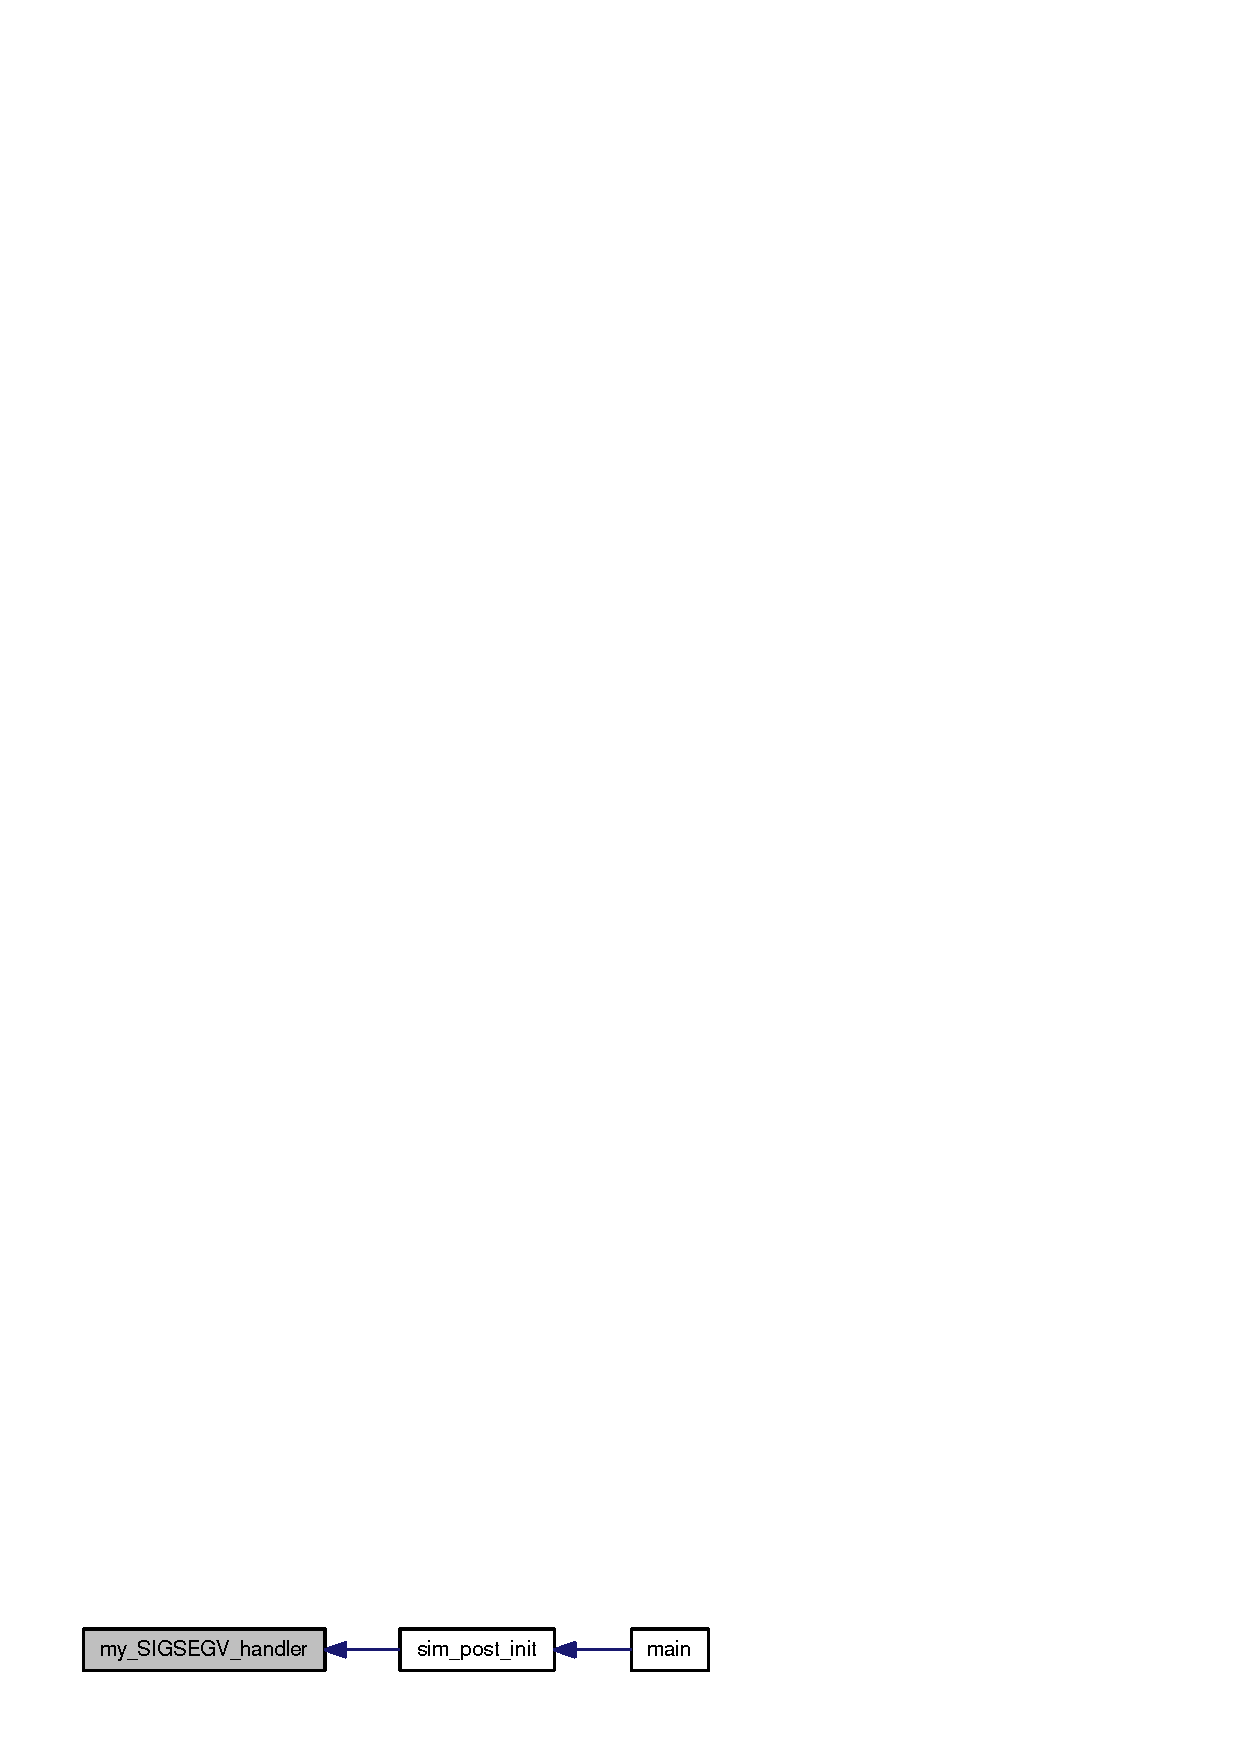
\includegraphics[width=172pt]{sim-zesto_8cpp_b35cfeccf968c0e4d7ce20475c5b8b69_icgraph}
\end{center}
\end{figure}
\index{sim-zesto.cpp@{sim-zesto.cpp}!sim\_\-aux\_\-config@{sim\_\-aux\_\-config}}
\index{sim\_\-aux\_\-config@{sim\_\-aux\_\-config}!sim-zesto.cpp@{sim-zesto.cpp}}
\subsubsection[{sim\_\-aux\_\-config}]{\setlength{\rightskip}{0pt plus 5cm}void sim\_\-aux\_\-config (FILE $\ast$ {\em stream})}\label{sim-zesto_8cpp_67e5d7a21600d2eb1fb2f0798fc24a7c}




Definition at line 423 of file sim-zesto.cpp.

Referenced by main().

Here is the caller graph for this function:\nopagebreak
\begin{figure}[H]
\begin{center}
\leavevmode
\includegraphics[width=101pt]{sim-zesto_8cpp_67e5d7a21600d2eb1fb2f0798fc24a7c_icgraph}
\end{center}
\end{figure}
\index{sim-zesto.cpp@{sim-zesto.cpp}!sim\_\-aux\_\-stats@{sim\_\-aux\_\-stats}}
\index{sim\_\-aux\_\-stats@{sim\_\-aux\_\-stats}!sim-zesto.cpp@{sim-zesto.cpp}}
\subsubsection[{sim\_\-aux\_\-stats}]{\setlength{\rightskip}{0pt plus 5cm}void sim\_\-aux\_\-stats (FILE $\ast$ {\em stream})}\label{sim-zesto_8cpp_f0d3b44eaaad1fd53b38c9f82deb05fd}




Definition at line 430 of file sim-zesto.cpp.

Referenced by sim\_\-print\_\-stats().

Here is the caller graph for this function:\nopagebreak
\begin{figure}[H]
\begin{center}
\leavevmode
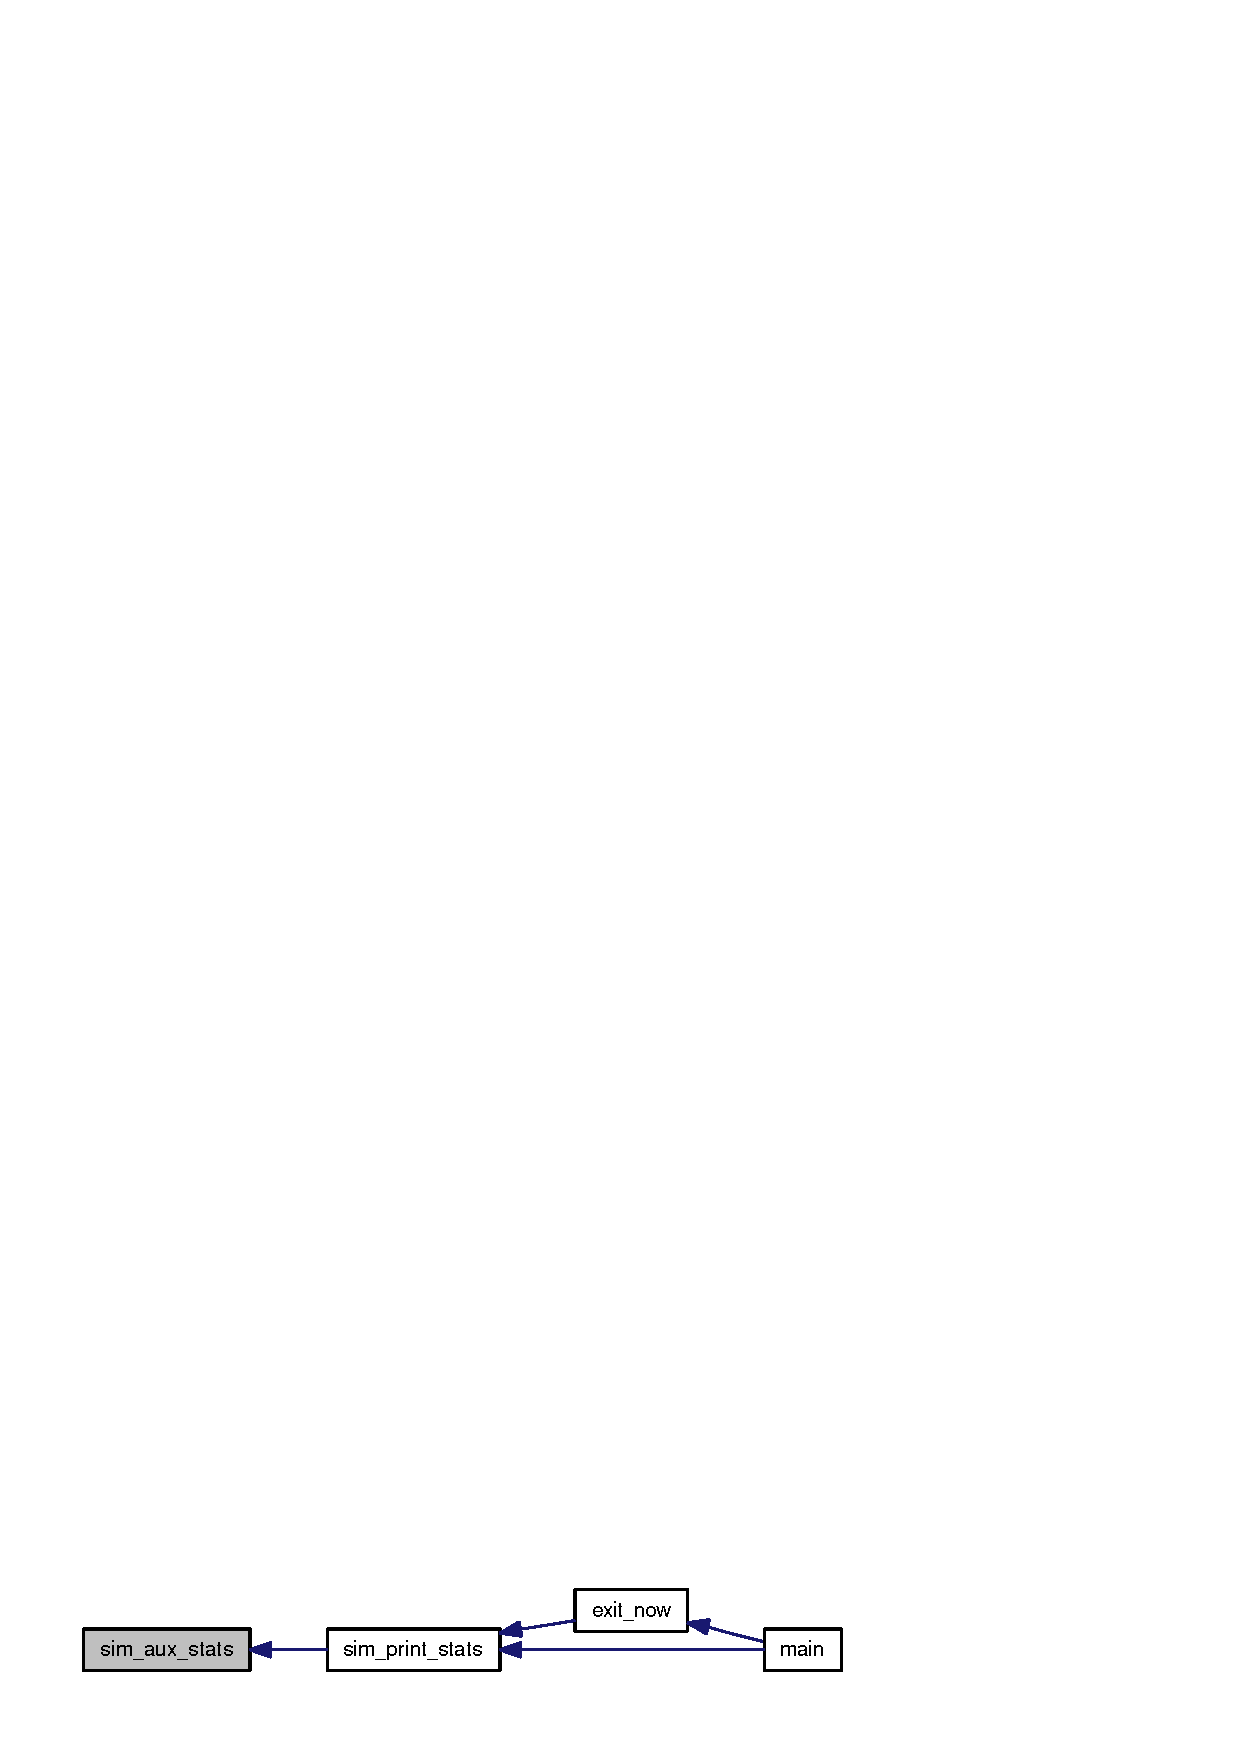
\includegraphics[width=204pt]{sim-zesto_8cpp_f0d3b44eaaad1fd53b38c9f82deb05fd_icgraph}
\end{center}
\end{figure}
\index{sim-zesto.cpp@{sim-zesto.cpp}!sim\_\-fastfwd@{sim\_\-fastfwd}}
\index{sim\_\-fastfwd@{sim\_\-fastfwd}!sim-zesto.cpp@{sim-zesto.cpp}}
\subsubsection[{sim\_\-fastfwd}]{\setlength{\rightskip}{0pt plus 5cm}void sim\_\-fastfwd (struct {\bf core\_\-t} $\ast$$\ast$ {\em cores}, \/  const unsigned int {\em insn\_\-count})}\label{sim-zesto_8cpp_d4465337904f2c1d2b694eb41043de6e}




Definition at line 634 of file sim-zesto.cpp.

References core\_\-fetch\_\-t::bpred, Mop\_\-t::bpred\_\-update, cache\_\-get\_\-evictee(), cache\_\-get\_\-evictee\_\-llc(), cache\_\-insert\_\-block(), cache\_\-insert\_\-block\_\-llc(), cache\_\-is\_\-hit(), cache\_\-is\_\-hit\_\-llc(), CACHE\_\-READ, cache\_\-reset\_\-stats(), CACHE\_\-WRITE, core\_\-t::current\_\-thread, Mop\_\-t::decode, cache\_\-line\_\-t::dirty, core\_\-t::core\_\-t::core\_\-memory\_\-t::DL1, core\_\-t::core\_\-t::core\_\-memory\_\-t::DL2, core\_\-t::core\_\-t::core\_\-memory\_\-t::DTLB, core\_\-t::core\_\-t::core\_\-memory\_\-t::DTLB2, core\_\-t::core\_\-t::core\_\-stat\_\-t::eio\_\-commit\_\-insn, F\_\-CTRL, F\_\-MEM, F\_\-STORE, F\_\-TRAP, core\_\-t::fetch, Mop\_\-t::fetch, core\_\-knobs\_\-t::fetch, bpred\_\-t::get\_\-state\_\-cache(), thread\_\-t::id, core\_\-t::id, core\_\-t::core\_\-t::core\_\-memory\_\-t::IL1, md\_\-inst\_\-t::imm, Mop\_\-t::inst, Mop\_\-t::is\_\-ctrl, Mop\_\-t::is\_\-trap, core\_\-t::core\_\-t::core\_\-memory\_\-t::ITLB, knobs, md\_\-inst\_\-t::len, uncore\_\-t::LLC, bpred\_\-t::lookup(), md\_\-fault\_\-none, MD\_\-FETCH\_\-INST, MD\_\-FETCH\_\-NEXT\_\-PC, MD\_\-INST\_\-SIZE, MD\_\-OP\_\-FLAGS, MD\_\-SET\_\-OPCODE\_\-DURING\_\-FETCH, thread\_\-t::mem, md\_\-inst\_\-t::mem\_\-paddr, md\_\-inst\_\-t::mem\_\-vaddr, core\_\-t::memory, core\_\-knobs\_\-t::memory, memzero(), Mop\_\-t::NextPC, no\_\-mcs, no\_\-nodes, thread\_\-t::num\_\-insn, num\_\-threads, Mop\_\-t::op, Mop\_\-t::opflags, Mop\_\-t::oracle, md\_\-inst\_\-t::paddr, PAGE\_\-TABLE\_\-ADDR, core\_\-fetch\_\-t::PC, Mop\_\-t::PC, bpred\_\-t::recover(), thread\_\-t::regs, regs\_\-t::regs\_\-NPC, regs\_\-t::regs\_\-PC, md\_\-inst\_\-t::rep, bpred\_\-t::reset\_\-stats(), bpred\_\-t::return\_\-state\_\-cache(), core\_\-t::stat, thread\_\-t::stat, Mop\_\-t::targetPC, core\_\-t::uncore, bpred\_\-t::update(), md\_\-inst\_\-t::vaddr, cache\_\-line\_\-t::valid, core\_\-knobs\_\-t::warm\_\-bpred, and core\_\-knobs\_\-t::warm\_\-caches.

Referenced by sim\_\-main().

Here is the caller graph for this function:\nopagebreak
\begin{figure}[H]
\begin{center}
\leavevmode
\includegraphics[width=141pt]{sim-zesto_8cpp_d4465337904f2c1d2b694eb41043de6e_icgraph}
\end{center}
\end{figure}
\index{sim-zesto.cpp@{sim-zesto.cpp}!sim\_\-main@{sim\_\-main}}
\index{sim\_\-main@{sim\_\-main}!sim-zesto.cpp@{sim-zesto.cpp}}
\subsubsection[{sim\_\-main}]{\setlength{\rightskip}{0pt plus 5cm}void sim\_\-main (void)}\label{sim-zesto_8cpp_6b9951fa76e6d8b400f13df1c975ed3b}




Definition at line 1006 of file sim-zesto.cpp.

References core\_\-t::current\_\-thread, fastfwd, fatal(), core\_\-t::fetch, MD\_\-FETCH\_\-NEXT\_\-PC, num\_\-threads, core\_\-fetch\_\-t::PC, thread\_\-t::pin\_\-trace, thread\_\-t::regs, regs\_\-t::regs\_\-NPC, regs\_\-t::regs\_\-PC, sim\_\-fastfwd(), sim\_\-start\_\-time, store\_\-nextPC, and use\_\-stored\_\-nextPC.

Referenced by main().

Here is the caller graph for this function:\nopagebreak
\begin{figure}[H]
\begin{center}
\leavevmode
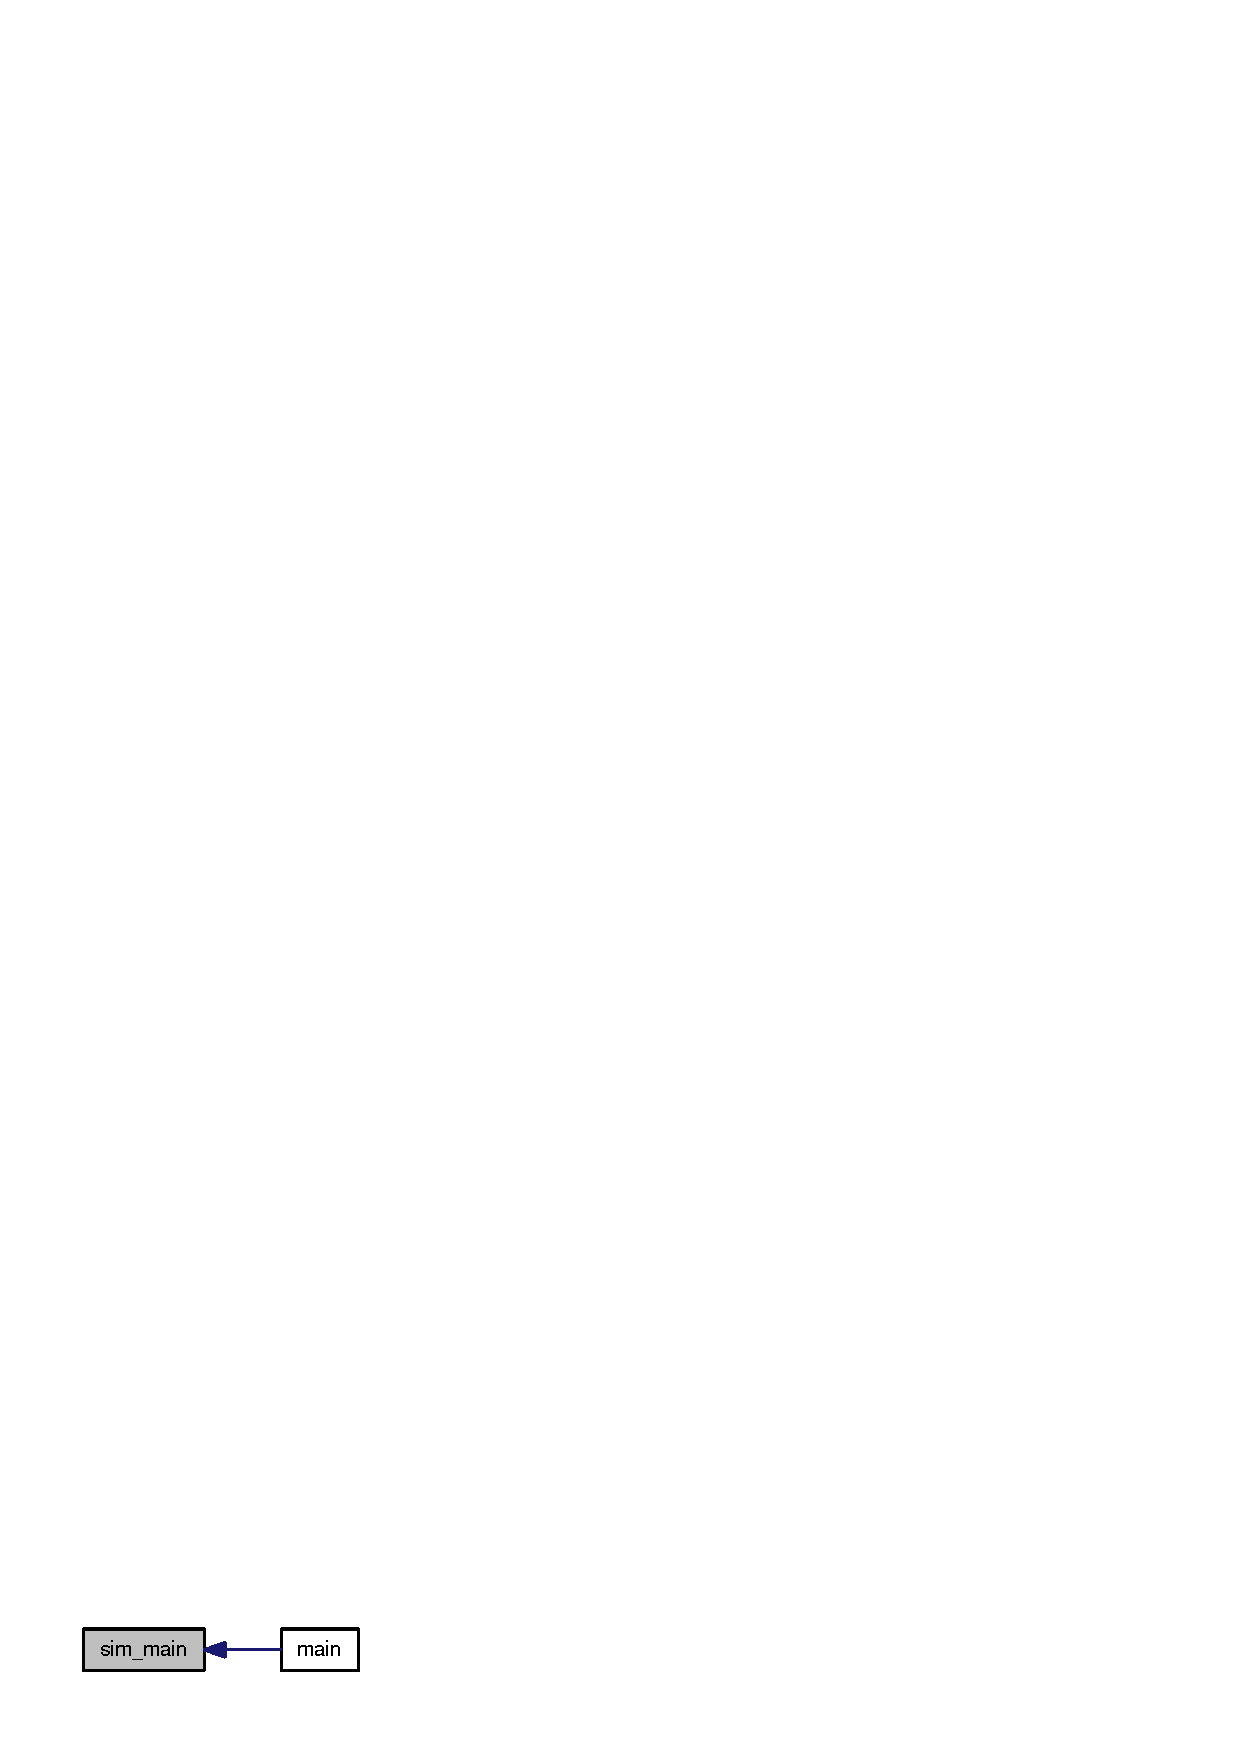
\includegraphics[width=88pt]{sim-zesto_8cpp_6b9951fa76e6d8b400f13df1c975ed3b_icgraph}
\end{center}
\end{figure}
\index{sim-zesto.cpp@{sim-zesto.cpp}!sim\_\-post\_\-init@{sim\_\-post\_\-init}}
\index{sim\_\-post\_\-init@{sim\_\-post\_\-init}!sim-zesto.cpp@{sim-zesto.cpp}}
\subsubsection[{sim\_\-post\_\-init}]{\setlength{\rightskip}{0pt plus 5cm}void sim\_\-post\_\-init (void)}\label{sim-zesto_8cpp_7af633ff74aee8f90ea9a610892191ce}




Definition at line 330 of file sim-zesto.cpp.

References thread\_\-t::active, core\_\-t::alloc, alloc\_\-create(), BOOT\_\-PC, core\_\-t::commit, commit\_\-create(), uncore\_\-t::core, core\_\-t::core\_\-t(), cores\_\-per\_\-node, cpu\_\-speed, thread\_\-t::current\_\-core, core\_\-t::current\_\-thread, core\_\-t::decode, decode\_\-create(), core\_\-t::exec, exec\_\-create(), fatal(), core\_\-t::fetch, fetch\_\-create(), thread\_\-t::id, knobs, core\_\-t::knobs, core\_\-knobs\_\-t::model, my\_\-SIGSEGV\_\-handler(), no\_\-mcs, no\_\-nodes, num\_\-threads, core\_\-t::oracle, thread\_\-t::regs, regs\_\-init(), regs\_\-t::regs\_\-PC, core\_\-t::uncore, uncore\_\-t::uncore\_\-t(), and vcs.

Referenced by main().

Here is the caller graph for this function:\nopagebreak
\begin{figure}[H]
\begin{center}
\leavevmode
\includegraphics[width=96pt]{sim-zesto_8cpp_7af633ff74aee8f90ea9a610892191ce_icgraph}
\end{center}
\end{figure}
\index{sim-zesto.cpp@{sim-zesto.cpp}!sim\_\-pre\_\-init@{sim\_\-pre\_\-init}}
\index{sim\_\-pre\_\-init@{sim\_\-pre\_\-init}!sim-zesto.cpp@{sim-zesto.cpp}}
\subsubsection[{sim\_\-pre\_\-init}]{\setlength{\rightskip}{0pt plus 5cm}void sim\_\-pre\_\-init (void)}\label{sim-zesto_8cpp_6f8bfcc0d1d039d6fb378af082656f6f}




Definition at line 193 of file sim-zesto.cpp.

References core\_\-knobs\_\-t::alloc, core\_\-knobs\_\-t::bpred\_\-opt\_\-str, core\_\-knobs\_\-t::branch\_\-decode\_\-limit, core\_\-knobs\_\-t::byteQ\_\-linesize, core\_\-knobs\_\-t::byteQ\_\-size, core\_\-knobs\_\-t::commit, core\_\-knobs\_\-t::decode, core\_\-knobs\_\-t::decoders, core\_\-knobs\_\-t::depth, core\_\-knobs\_\-t::DL1\_\-MSHR\_\-cmd, core\_\-knobs\_\-t::DL1\_\-num\_\-PF, core\_\-knobs\_\-t::DL1PF\_\-opt\_\-str, core\_\-knobs\_\-t::DL2\_\-MSHR\_\-cmd, core\_\-knobs\_\-t::DL2\_\-num\_\-PF, core\_\-knobs\_\-t::DL2PF\_\-opt\_\-str, core\_\-knobs\_\-t::exec, core\_\-knobs\_\-t::fetch, core\_\-knobs\_\-t::fp\_\-penalty, core\_\-knobs\_\-t::fu\_\-bindings, FU\_\-FADD, FU\_\-FCPLX, FU\_\-FDIV, FU\_\-FMUL, FU\_\-IDIV, FU\_\-IEU, FU\_\-IMUL, FU\_\-JEU, FU\_\-LD, FU\_\-SHIFT, FU\_\-STA, FU\_\-STD, core\_\-knobs\_\-t::IL1\_\-num\_\-PF, core\_\-knobs\_\-t::IL1PF\_\-opt\_\-str, core\_\-knobs\_\-t::IQ\_\-size, core\_\-knobs\_\-t::issue\_\-rate, knobs, core\_\-knobs\_\-t::latency, core\_\-knobs\_\-t::LDQ\_\-size, MAX\_\-DECODE\_\-WIDTH, core\_\-knobs\_\-t::memory, memzero(), core\_\-knobs\_\-t::model, core\_\-knobs\_\-t::MS\_\-latency, core\_\-knobs\_\-t::num\_\-bpred\_\-components, core\_\-knobs\_\-t::num\_\-decoder\_\-specs, core\_\-knobs\_\-t::num\_\-exec\_\-ports, core\_\-knobs\_\-t::payload\_\-depth, core\_\-knobs\_\-t::port\_\-binding, core\_\-knobs\_\-t::ROB\_\-size, core\_\-knobs\_\-t::RS\_\-size, core\_\-knobs\_\-t::STQ\_\-size, core\_\-knobs\_\-t::target\_\-stage, core\_\-knobs\_\-t::uopQ\_\-size, and core\_\-knobs\_\-t::width.

Referenced by main().

Here is the caller graph for this function:\nopagebreak
\begin{figure}[H]
\begin{center}
\leavevmode
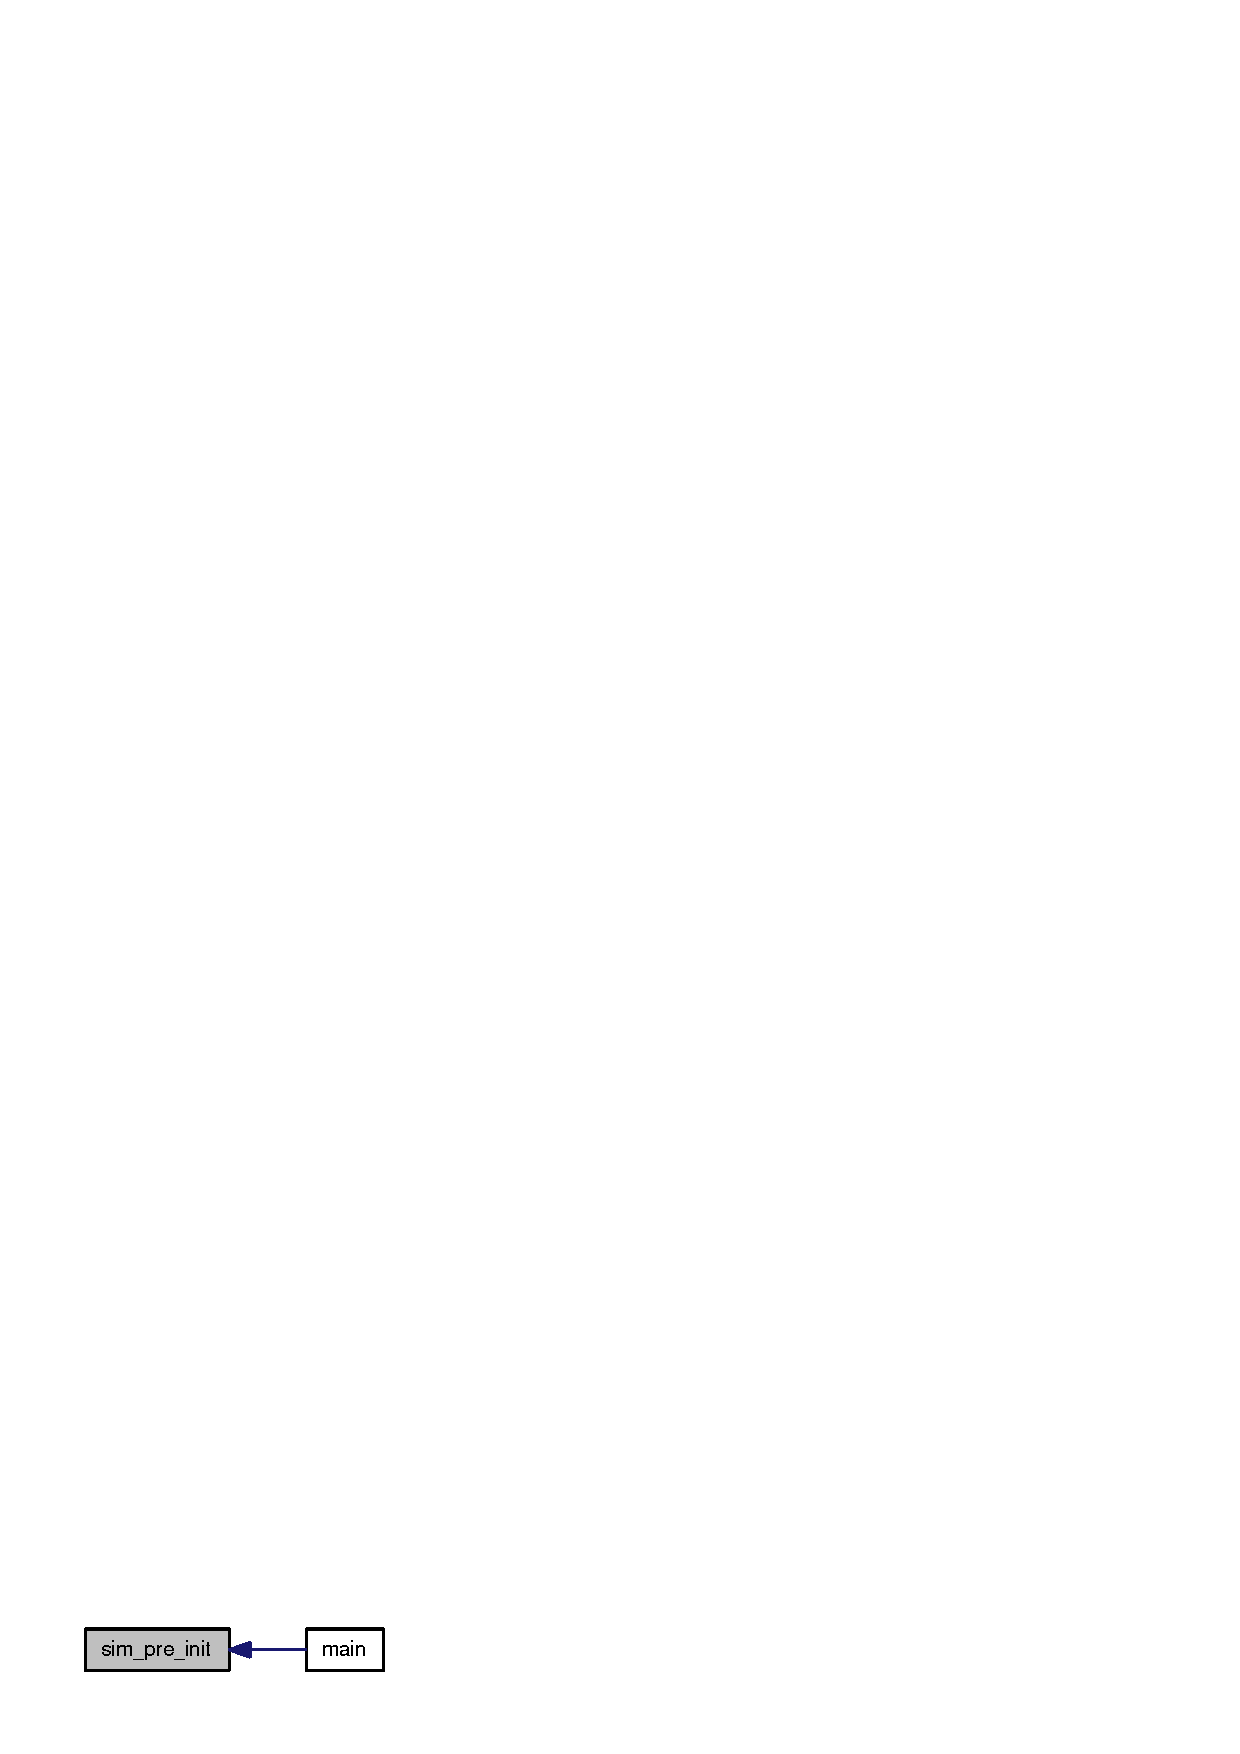
\includegraphics[width=94pt]{sim-zesto_8cpp_6f8bfcc0d1d039d6fb378af082656f6f_icgraph}
\end{center}
\end{figure}
\index{sim-zesto.cpp@{sim-zesto.cpp}!sim\_\-uninit@{sim\_\-uninit}}
\index{sim\_\-uninit@{sim\_\-uninit}!sim-zesto.cpp@{sim-zesto.cpp}}
\subsubsection[{sim\_\-uninit}]{\setlength{\rightskip}{0pt plus 5cm}void sim\_\-uninit (void)}\label{sim-zesto_8cpp_12f418d794abd0896d834c9582373b00}




Definition at line 437 of file sim-zesto.cpp.

Referenced by exit\_\-now().

Here is the caller graph for this function:\nopagebreak
\begin{figure}[H]
\begin{center}
\leavevmode
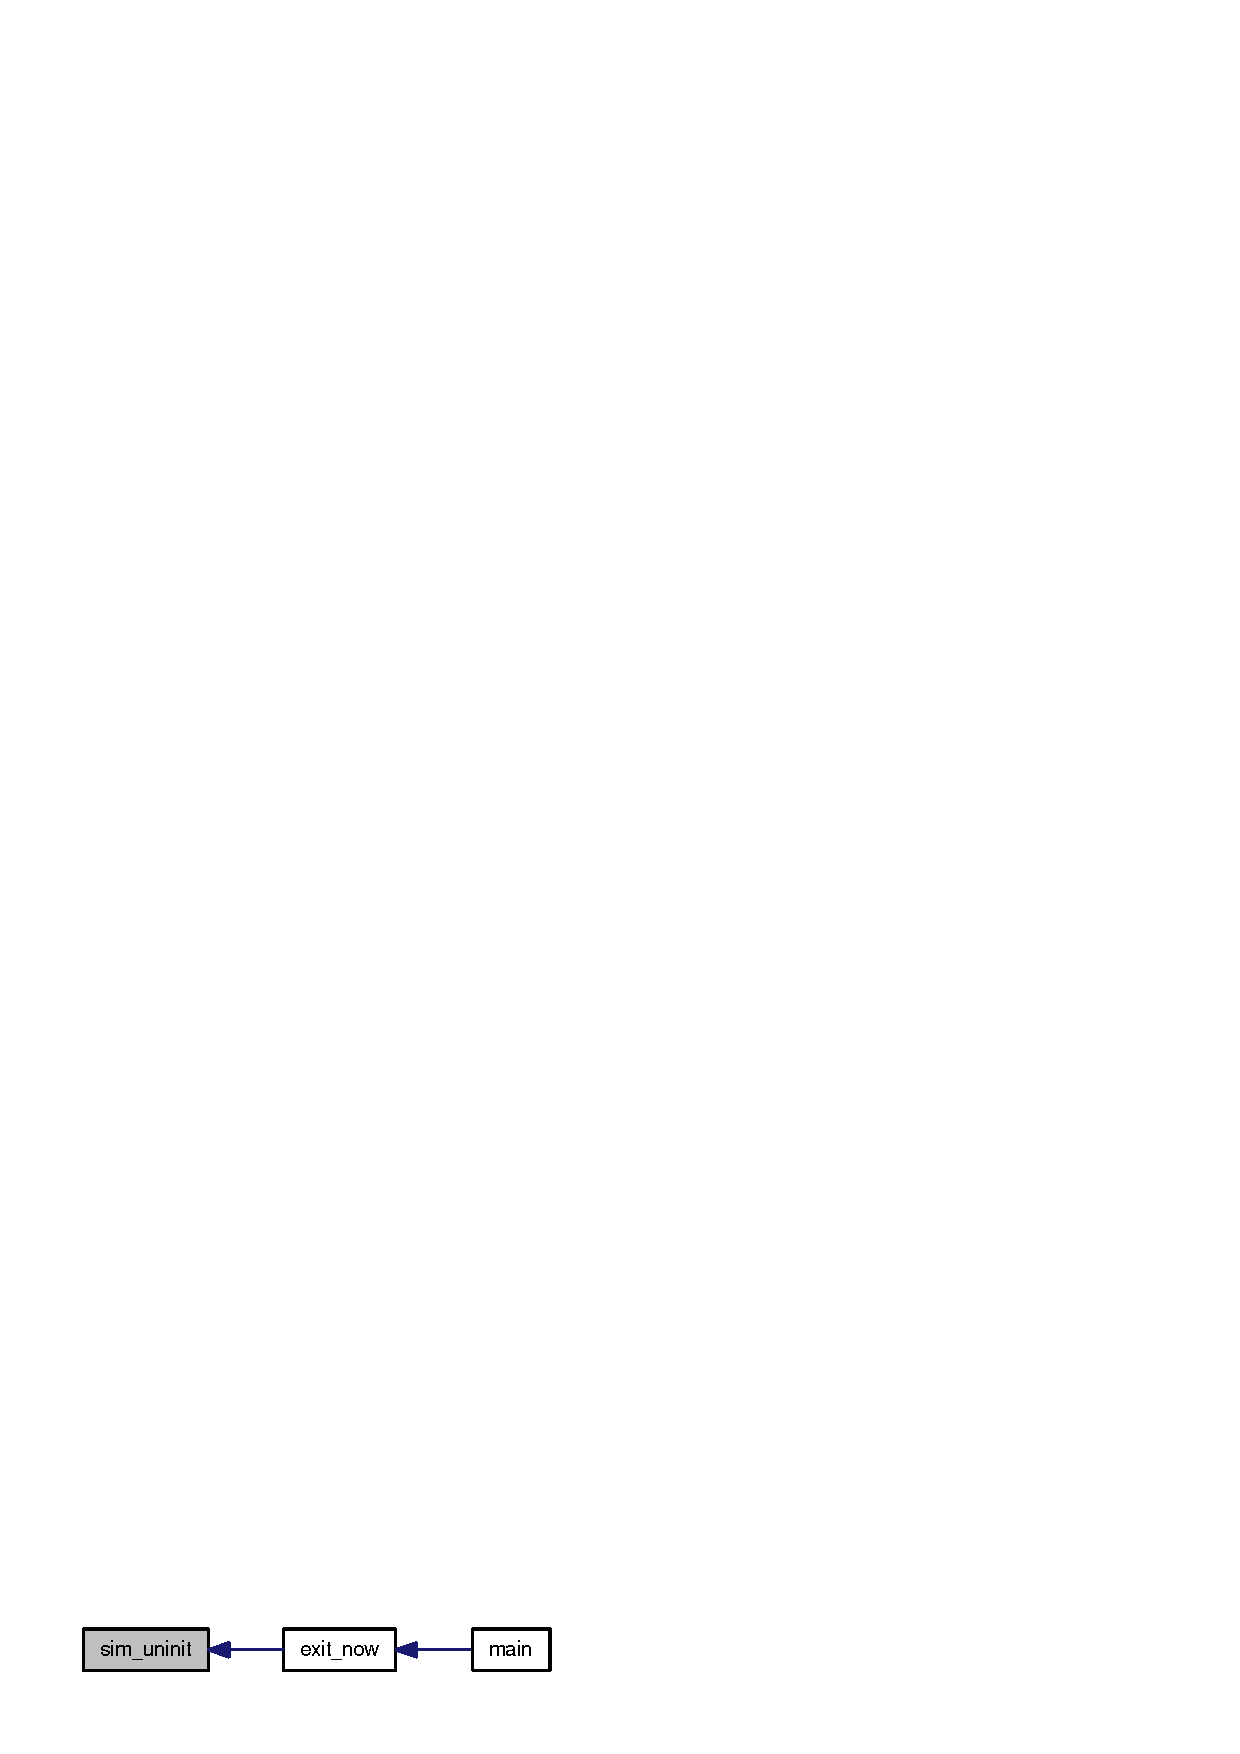
\includegraphics[width=134pt]{sim-zesto_8cpp_12f418d794abd0896d834c9582373b00_icgraph}
\end{center}
\end{figure}


\subsection{Variable Documentation}
\index{sim-zesto.cpp@{sim-zesto.cpp}!cores@{cores}}
\index{cores@{cores}!sim-zesto.cpp@{sim-zesto.cpp}}
\subsubsection[{cores}]{\setlength{\rightskip}{0pt plus 5cm}struct {\bf core\_\-t}$\ast$$\ast$ {\bf cores} = NULL}\label{sim-zesto_8cpp_fd1fbe748ceabf38ef289bb5b346f69a}




Definition at line 170 of file sim-zesto.cpp.

Referenced by md\_\-fetch\_\-inst(), md\_\-fetch\_\-next\_\-pc(), and core\_\-oracle\_\-t::syscall\_\-mem\_\-access().\index{sim-zesto.cpp@{sim-zesto.cpp}!cpu\_\-speed@{cpu\_\-speed}}
\index{cpu\_\-speed@{cpu\_\-speed}!sim-zesto.cpp@{sim-zesto.cpp}}
\subsubsection[{cpu\_\-speed}]{\setlength{\rightskip}{0pt plus 5cm}double {\bf cpu\_\-speed} = 3000}\label{sim-zesto_8cpp_ebb0be7596a98356724d9653c17116c2}




Definition at line 176 of file sim-zesto.cpp.

Referenced by sim\_\-post\_\-init(), and uncore\_\-reg\_\-options().\index{sim-zesto.cpp@{sim-zesto.cpp}!heartbeat\_\-count@{heartbeat\_\-count}}
\index{heartbeat\_\-count@{heartbeat\_\-count}!sim-zesto.cpp@{sim-zesto.cpp}}
\subsubsection[{heartbeat\_\-count}]{\setlength{\rightskip}{0pt plus 5cm}int {\bf heartbeat\_\-count} = 0}\label{sim-zesto_8cpp_af9443448449d3e516d9e748c4fbb6bf}




Definition at line 181 of file sim-zesto.cpp.

Referenced by zesto\_\-component::downtick\_\-handler().\index{sim-zesto.cpp@{sim-zesto.cpp}!knobs@{knobs}}
\index{knobs@{knobs}!sim-zesto.cpp@{sim-zesto.cpp}}
\subsubsection[{knobs}]{\setlength{\rightskip}{0pt plus 5cm}struct {\bf core\_\-knobs\_\-t} {\bf knobs}}\label{sim-zesto_8cpp_89a180011adecec49b08c8ef843388fa}




Definition at line 183 of file sim-zesto.cpp.

Referenced by core\_\-exec\_\-STM\_\-t::ALU\_\-exec(), core\_\-exec\_\-DPM\_\-t::ALU\_\-exec(), core\_\-fetch\_\-STM\_\-t::byteQ\_\-already\_\-requested(), core\_\-fetch\_\-DPM\_\-t::byteQ\_\-already\_\-requested(), core\_\-fetch\_\-STM\_\-t::byteQ\_\-is\_\-full(), core\_\-fetch\_\-DPM\_\-t::byteQ\_\-is\_\-full(), core\_\-fetch\_\-STM\_\-t::byteQ\_\-request(), core\_\-fetch\_\-DPM\_\-t::byteQ\_\-request(), core\_\-decode\_\-STM\_\-t::check\_\-flush(), core\_\-decode\_\-DPM\_\-t::check\_\-flush(), core\_\-exec\_\-STM\_\-t::check\_\-load\_\-issue\_\-conditions(), core\_\-exec\_\-DPM\_\-t::check\_\-load\_\-issue\_\-conditions(), core\_\-alloc\_\-DPM\_\-t::core\_\-alloc\_\-DPM\_\-t(), core\_\-alloc\_\-STM\_\-t::core\_\-alloc\_\-STM\_\-t(), core\_\-commit\_\-DPM\_\-t::core\_\-commit\_\-DPM\_\-t(), core\_\-commit\_\-STM\_\-t::core\_\-commit\_\-STM\_\-t(), core\_\-decode\_\-DPM\_\-t::core\_\-decode\_\-DPM\_\-t(), core\_\-decode\_\-STM\_\-t::core\_\-decode\_\-STM\_\-t(), core\_\-exec\_\-DPM\_\-t::core\_\-exec\_\-DPM\_\-t(), core\_\-exec\_\-STM\_\-t::core\_\-exec\_\-STM\_\-t(), core\_\-fetch\_\-DPM\_\-t::core\_\-fetch\_\-DPM\_\-t(), core\_\-fetch\_\-STM\_\-t::core\_\-fetch\_\-STM\_\-t(), core\_\-oracle\_\-t::core\_\-oracle\_\-t(), core\_\-oracle\_\-t::exec(), core\_\-exec\_\-STM\_\-t::insert\_\-ready\_\-uop(), core\_\-exec\_\-DPM\_\-t::insert\_\-ready\_\-uop(), core\_\-exec\_\-STM\_\-t::LDQ\_\-available(), core\_\-exec\_\-DPM\_\-t::LDQ\_\-available(), core\_\-exec\_\-STM\_\-t::LDQ\_\-deallocate(), core\_\-exec\_\-DPM\_\-t::LDQ\_\-deallocate(), core\_\-exec\_\-STM\_\-t::LDQ\_\-insert(), core\_\-exec\_\-DPM\_\-t::LDQ\_\-insert(), core\_\-exec\_\-STM\_\-t::LDQ\_\-schedule(), core\_\-exec\_\-DPM\_\-t::LDQ\_\-schedule(), core\_\-exec\_\-STM\_\-t::LDQ\_\-squash(), core\_\-exec\_\-DPM\_\-t::LDQ\_\-squash(), core\_\-exec\_\-STM\_\-t::LDST\_\-exec(), core\_\-exec\_\-DPM\_\-t::LDST\_\-exec(), core\_\-exec\_\-DPM\_\-t::load\_\-miss\_\-reschedule(), core\_\-exec\_\-STM\_\-t::load\_\-writeback(), core\_\-exec\_\-DPM\_\-t::load\_\-writeback(), core\_\-fetch\_\-STM\_\-t::Mop\_\-consume(), core\_\-fetch\_\-DPM\_\-t::Mop\_\-consume(), core\_\-oracle\_\-t::pipe\_\-recover(), core\_\-fetch\_\-DPM\_\-t::predecode\_\-enqueue(), core\_\-fetch\_\-STM\_\-t::recover(), core\_\-fetch\_\-DPM\_\-t::recover(), core\_\-decode\_\-STM\_\-t::recover(), core\_\-decode\_\-DPM\_\-t::recover(), core\_\-commit\_\-STM\_\-t::recover(), core\_\-commit\_\-DPM\_\-t::recover(), core\_\-alloc\_\-DPM\_\-t::recover(), core\_\-decode\_\-DPM\_\-t::recover\_\-decode\_\-pipe(), core\_\-decode\_\-DPM\_\-t::recover\_\-uopQ(), core\_\-commit\_\-STM\_\-t::ROB\_\-available(), core\_\-commit\_\-DPM\_\-t::ROB\_\-available(), core\_\-commit\_\-STM\_\-t::ROB\_\-insert(), core\_\-commit\_\-DPM\_\-t::ROB\_\-insert(), core\_\-exec\_\-STM\_\-t::RS\_\-available(), core\_\-exec\_\-DPM\_\-t::RS\_\-available(), core\_\-exec\_\-STM\_\-t::RS\_\-deallocate(), core\_\-exec\_\-DPM\_\-t::RS\_\-deallocate(), core\_\-exec\_\-STM\_\-t::RS\_\-insert(), core\_\-exec\_\-DPM\_\-t::RS\_\-insert(), core\_\-exec\_\-STM\_\-t::RS\_\-schedule(), core\_\-exec\_\-DPM\_\-t::RS\_\-schedule(), sim\_\-fastfwd(), sim\_\-post\_\-init(), sim\_\-pre\_\-init(), core\_\-exec\_\-DPM\_\-t::snatch\_\-back(), core\_\-fetch\_\-STM\_\-t::step(), core\_\-fetch\_\-DPM\_\-t::step(), core\_\-decode\_\-STM\_\-t::step(), core\_\-decode\_\-DPM\_\-t::step(), core\_\-commit\_\-STM\_\-t::step(), core\_\-commit\_\-DPM\_\-t::step(), core\_\-alloc\_\-STM\_\-t::step(), core\_\-alloc\_\-DPM\_\-t::step(), core\_\-exec\_\-STM\_\-t::store\_\-dl1\_\-callback(), core\_\-exec\_\-DPM\_\-t::store\_\-dl1\_\-callback(), core\_\-exec\_\-DPM\_\-t::store\_\-dl1\_\-split\_\-callback(), core\_\-exec\_\-STM\_\-t::store\_\-dtlb\_\-callback(), core\_\-exec\_\-DPM\_\-t::store\_\-dtlb\_\-callback(), core\_\-exec\_\-DPM\_\-t::store\_\-translated\_\-callback(), core\_\-exec\_\-STM\_\-t::STQ\_\-available(), core\_\-exec\_\-DPM\_\-t::STQ\_\-available(), core\_\-exec\_\-DPM\_\-t::STQ\_\-deallocate\_\-senior(), core\_\-exec\_\-STM\_\-t::STQ\_\-deallocate\_\-std(), core\_\-exec\_\-DPM\_\-t::STQ\_\-deallocate\_\-std(), core\_\-exec\_\-STM\_\-t::STQ\_\-insert\_\-sta(), core\_\-exec\_\-DPM\_\-t::STQ\_\-insert\_\-sta(), core\_\-exec\_\-STM\_\-t::STQ\_\-insert\_\-std(), core\_\-exec\_\-DPM\_\-t::STQ\_\-insert\_\-std(), core\_\-exec\_\-DPM\_\-t::STQ\_\-squash\_\-senior(), core\_\-exec\_\-STM\_\-t::STQ\_\-squash\_\-sta(), core\_\-exec\_\-DPM\_\-t::STQ\_\-squash\_\-sta(), core\_\-exec\_\-STM\_\-t::STQ\_\-squash\_\-std(), core\_\-exec\_\-DPM\_\-t::STQ\_\-squash\_\-std(), core\_\-decode\_\-STM\_\-t::uop\_\-available(), core\_\-decode\_\-STM\_\-t::uop\_\-consume(), core\_\-decode\_\-DPM\_\-t::uop\_\-consume(), and core\_\-decode\_\-STM\_\-t::uop\_\-peek().\index{sim-zesto.cpp@{sim-zesto.cpp}!num\_\-threads@{num\_\-threads}}
\index{num\_\-threads@{num\_\-threads}!sim-zesto.cpp@{sim-zesto.cpp}}
\subsubsection[{num\_\-threads}]{\setlength{\rightskip}{0pt plus 5cm}unsigned int {\bf num\_\-threads} = 1}\label{sim-zesto_8cpp_26a8352e9cd3bc9a6a35bc8d88152985}




Definition at line 186 of file sim-zesto.cpp.

Referenced by cache\_\-create(), cache\_\-create\_\-llc(), cache\_\-reset\_\-stats(), zesto\_\-component::downtick\_\-handler(), LLC\_\-reg\_\-stats(), main(), sim\_\-fastfwd(), sim\_\-main(), and sim\_\-post\_\-init().\index{sim-zesto.cpp@{sim-zesto.cpp}!sim\_\-cycle@{sim\_\-cycle}}
\index{sim\_\-cycle@{sim\_\-cycle}!sim-zesto.cpp@{sim-zesto.cpp}}
\subsubsection[{sim\_\-cycle}]{\setlength{\rightskip}{0pt plus 5cm}{\bf tick\_\-t} {\bf sim\_\-cycle} = 0}\label{sim-zesto_8cpp_d93be82106e505ae03e3a443a62d7238}




Definition at line 189 of file sim-zesto.cpp.

Referenced by core\_\-exec\_\-STM\_\-t::ALU\_\-exec(), core\_\-exec\_\-DPM\_\-t::ALU\_\-exec(), bus\_\-free(), bus\_\-use(), cache\_\-enqueue(), cache\_\-enqueue\_\-llc(), cache\_\-fill(), cache\_\-fill\_\-llc(), cache\_\-process(), cache\_\-process\_\-llc(), core\_\-exec\_\-STM\_\-t::DL1\_\-callback(), core\_\-exec\_\-DPM\_\-t::DL1\_\-callback(), core\_\-exec\_\-DPM\_\-t::DL1\_\-split\_\-callback(), zesto\_\-component::downtick\_\-handler(), core\_\-exec\_\-STM\_\-t::DTLB\_\-callback(), core\_\-exec\_\-DPM\_\-t::DTLB\_\-callback(), uncore\_\-t::enqueue(), fill\_\-arrived(), fill\_\-arrived\_\-llc(), core\_\-exec\_\-STM\_\-t::get\_\-readyQ\_\-node(), core\_\-exec\_\-DPM\_\-t::get\_\-readyQ\_\-node(), GlobalAddrRip(), core\_\-fetch\_\-STM\_\-t::IL1\_\-callback(), core\_\-fetch\_\-DPM\_\-t::IL1\_\-callback(), core\_\-fetch\_\-STM\_\-t::ITLB\_\-callback(), core\_\-fetch\_\-DPM\_\-t::ITLB\_\-callback(), core\_\-exec\_\-STM\_\-t::LDQ\_\-schedule(), core\_\-exec\_\-DPM\_\-t::LDQ\_\-schedule(), core\_\-exec\_\-STM\_\-t::LDST\_\-exec(), core\_\-exec\_\-DPM\_\-t::LDST\_\-exec(), core\_\-exec\_\-DPM\_\-t::load\_\-miss\_\-reschedule(), core\_\-exec\_\-STM\_\-t::load\_\-writeback(), core\_\-exec\_\-DPM\_\-t::load\_\-writeback(), core\_\-fetch\_\-STM\_\-t::Mop\_\-consume(), my\_\-SIGSEGV\_\-handler(), prefetch\_\-controller\_\-update(), prefetch\_\-controller\_\-update\_\-llc(), prefetch\_\-filter\_\-lookup(), prefetch\_\-filter\_\-update(), core\_\-exec\_\-STM\_\-t::RS\_\-schedule(), core\_\-exec\_\-DPM\_\-t::RS\_\-schedule(), core\_\-fetch\_\-STM\_\-t::step(), core\_\-fetch\_\-DPM\_\-t::step(), core\_\-decode\_\-DPM\_\-t::step(), core\_\-commit\_\-STM\_\-t::step(), core\_\-commit\_\-DPM\_\-t::step(), core\_\-alloc\_\-STM\_\-t::step(), core\_\-alloc\_\-DPM\_\-t::step(), core\_\-fetch\_\-STM\_\-t::translated\_\-callback(), core\_\-fetch\_\-DPM\_\-t::translated\_\-callback(), core\_\-exec\_\-STM\_\-t::translated\_\-callback(), core\_\-exec\_\-DPM\_\-t::translated\_\-callback(), and core\_\-decode\_\-STM\_\-t::uop\_\-consume().\index{sim-zesto.cpp@{sim-zesto.cpp}!simulated\_\-processes\_\-remaining@{simulated\_\-processes\_\-remaining}}
\index{simulated\_\-processes\_\-remaining@{simulated\_\-processes\_\-remaining}!sim-zesto.cpp@{sim-zesto.cpp}}
\subsubsection[{simulated\_\-processes\_\-remaining}]{\setlength{\rightskip}{0pt plus 5cm}int {\bf simulated\_\-processes\_\-remaining} = 1}\label{sim-zesto_8cpp_1b2701dab57f1ffb6459bbde33452d68}




Definition at line 187 of file sim-zesto.cpp.

Referenced by core\_\-commit\_\-STM\_\-t::step(), and core\_\-commit\_\-DPM\_\-t::step().\index{sim-zesto.cpp@{sim-zesto.cpp}!start\_\-pos@{start\_\-pos}}
\index{start\_\-pos@{start\_\-pos}!sim-zesto.cpp@{sim-zesto.cpp}}
\subsubsection[{start\_\-pos}]{\setlength{\rightskip}{0pt plus 5cm}int {\bf start\_\-pos} = 0}\label{sim-zesto_8cpp_9715e2df77829e54cb078a298fd6c434}




Definition at line 179 of file sim-zesto.cpp.

Referenced by zesto\_\-component::downtick\_\-handler().\index{sim-zesto.cpp@{sim-zesto.cpp}!store\_\-nextPC@{store\_\-nextPC}}
\index{store\_\-nextPC@{store\_\-nextPC}!sim-zesto.cpp@{sim-zesto.cpp}}
\subsubsection[{store\_\-nextPC}]{\setlength{\rightskip}{0pt plus 5cm}{\bf md\_\-addr\_\-t} {\bf store\_\-nextPC}[16]}\label{sim-zesto_8cpp_87de3dd0dc95ac44e817dc0f7c7ba3d7}




Definition at line 159 of file zesto-oracle.cpp.

Referenced by md\_\-fetch\_\-inst(), md\_\-fetch\_\-next\_\-pc(), core\_\-oracle\_\-t::pipe\_\-flush(), and sim\_\-main().\index{sim-zesto.cpp@{sim-zesto.cpp}!threads@{threads}}
\index{threads@{threads}!sim-zesto.cpp@{sim-zesto.cpp}}
\subsubsection[{threads}]{\setlength{\rightskip}{0pt plus 5cm}struct {\bf thread\_\-t}$\ast$$\ast$ {\bf threads} = NULL}\label{sim-zesto_8cpp_f227be61b1f91b71aafae105501d92f7}




Definition at line 167 of file sim-zesto.cpp.

Referenced by main(), and core\_\-oracle\_\-t::syscall\_\-mem\_\-access().\index{sim-zesto.cpp@{sim-zesto.cpp}!uncores@{uncores}}
\index{uncores@{uncores}!sim-zesto.cpp@{sim-zesto.cpp}}
\subsubsection[{uncores}]{\setlength{\rightskip}{0pt plus 5cm}struct {\bf uncore\_\-t}$\ast$$\ast$ {\bf uncores} = NULL}\label{sim-zesto_8cpp_58a16285046a9c04416e306f52015b52}




Definition at line 173 of file sim-zesto.cpp.

Referenced by iris\_\-init().\index{sim-zesto.cpp@{sim-zesto.cpp}!use\_\-stored\_\-nextPC@{use\_\-stored\_\-nextPC}}
\index{use\_\-stored\_\-nextPC@{use\_\-stored\_\-nextPC}!sim-zesto.cpp@{sim-zesto.cpp}}
\subsubsection[{use\_\-stored\_\-nextPC}]{\setlength{\rightskip}{0pt plus 5cm}bool {\bf use\_\-stored\_\-nextPC}[16]}\label{sim-zesto_8cpp_38a36f4cd3940833135cd0c497f726f4}




Definition at line 160 of file zesto-oracle.cpp.

Referenced by emergency\_\-recovery(), md\_\-fetch\_\-inst(), md\_\-fetch\_\-next\_\-pc(), and sim\_\-main().